%definira klasu dokumenta 
\documentclass[12pt]{report} 

%prostor izmedu naredbi \documentclass i \begin{document} se zove uvod. U njemu se nalaze naredbe koje se odnose na cijeli dokument

%osnovni LaTex ne može riješiti sve probleme, pa se koriste različiti paketi koji olakšavaju izradu željenog dokumenta
\usepackage[croatian]{babel} 
\usepackage{amssymb}
\usepackage{amsmath}
\usepackage{txfonts}
\usepackage{mathdots}
\usepackage{titlesec}
\usepackage{array}
\usepackage{lastpage}
\usepackage{etoolbox}
\usepackage{tabularray}
\usepackage{color, colortbl}
\usepackage{adjustbox}
\usepackage{geometry}
\usepackage[classicReIm]{kpfonts}
\usepackage{hyperref}
\usepackage{fancyhdr}

\usepackage{float}
\usepackage{setspace}
\restylefloat{table}


\patchcmd{\chapter}{\thispagestyle{plain}}{\thispagestyle{fancy}}{}{} %redefiniranje stila stranice u paketu fancyhdr

%oblik naslova poglavlja
\titleformat{\chapter}{\normalfont\huge\bfseries}{\thechapter.}{20pt}{\Huge}
\titlespacing{\chapter}{0pt}{0pt}{40pt}


\linespread{1.3} %razmak između redaka

\geometry{a4paper, left=1in, top=1in,}  %oblik stranice

\hypersetup{ colorlinks, citecolor=black, filecolor=black, linkcolor=black,	urlcolor=black }   %izgled poveznice


%prored smanjen između redaka u nabrajanjima i popisima
\newenvironment{packed_enum}{
	\begin{enumerate}
		\setlength{\itemsep}{0pt}
		\setlength{\parskip}{0pt}
		\setlength{\parsep}{0pt}
	}{\end{enumerate}}

\newenvironment{packed_item}{
	\begin{itemize}
		\setlength{\itemsep}{0pt}
		\setlength{\parskip}{0pt}
		\setlength{\parsep}{0pt}
	}{\end{itemize}}




%boja za privatni i udaljeni kljuc u tablicama
\definecolor{LightBlue}{rgb}{0.9,0.9,1}
\definecolor{LightGreen}{rgb}{0.9,1,0.9}

%Promjena teksta za dugačke tablice
\DefTblrTemplate{contfoot-text}{normal}{Nastavljeno na idućoj stranici}
\SetTblrTemplate{contfoot-text}{normal}
\DefTblrTemplate{conthead-text}{normal}{(Nastavljeno)}
\SetTblrTemplate{conthead-text}{normal}
\DefTblrTemplate{middlehead,lasthead}{normal}{Nastavljeno od prethodne stranice}
\SetTblrTemplate{middlehead,lasthead}{normal}

%podesavanje zaglavlja i podnožja

\pagestyle{fancy}
\lhead{Programsko inženjerstvo}
\rhead{WildTrack}
\lfoot{Pokret nesvrstanih}
\cfoot{stranica \thepage/\pageref{LastPage}}
\rfoot{\today}
\renewcommand{\headrulewidth}{0.2pt}
\renewcommand{\footrulewidth}{0.2pt}


\begin{document} 
	
	
	
	\begin{titlepage}
		\begin{center}
			\vspace*{\stretch{1.0}} %u kombinaciji s ostalim \vspace naredbama definira razmak između redaka teksta
			\LARGE Programsko inženjerstvo\\
			\large Ak. god. 2023./2024.\\
			
			\vspace*{\stretch{3.0}}
			
			\huge WildTrack\\
			\Large Dokumentacija, Rev. 0.10\\
			
			\vspace*{\stretch{12.0}}
			\normalsize
			Grupa: \textit{Pokret nesvrstanih}\\
			Voditelj: \textit{Emil Prpić}\\
			
			
			\vspace*{\stretch{1.0}}
			Datum predaje: \textit{$<$dan$>$. $<$mjesec$>$. $<$godina$>$.}\\
	
			\vspace*{\stretch{4.0}}
			
			Nastavnik: \textit{Hrvoje Nuić}\\
		
		\end{center}

	
	\end{titlepage}

	
	\tableofcontents


	\chapter{Dnevnik promjena dokumentacije}
		
		
				
		
		\begin{longtblr}[
				label=none
			]{
				width = \textwidth, 
				colspec={|X[2]|X[13]|X[3]|X[3]|}, 
				rowhead = 1
			}
			\hline
			\textbf{Rev.}	& \textbf{Opis promjene/dodatka} & \textbf{Autori} & \textbf{Datum}\\[3pt] \hline
			0.1 & Napravljen predložak.	& Sebastian Medjaković & 26.10.2023. 		\\[3pt] \hline 
			0.2	& Opis projekta i funkcionalni zahtjevi. & Sara Gašpar & 30.10.2023. 	\\[3pt] \hline
			0.3	& Nabrojeni obrasci uporabe & Sebastian Medjaković & 1.11.2023. 	\\[3pt] \hline
			0.4 & Opis obrazaca uporabe & svi & 1.11.2023. \\[3pt] \hline
			0.5 & Dodan model baze i nefunkcionalni zahtjevi & Sebastian Medjaković & 2.11.2023. \\[3pt] \hline 
			0.6 & Arhitektura i dizajn sustava & Sara Gašpar & 2.11.2023. \\[3pt] \hline 
			0.7 & Revizija dokumentacije & Sara Gašpar, Sebastian Medjaković & 2.11.2023. \\[3pt] \hline 
			0.8 & Dijagrami obrazaca uporabe & Jure Spajić, Filip Vitković & 06.11.2023. \\[3pt] \hline 
			0.9 & Sekvencijski dijagrami & Ivan Cvijetić, Filip Vitković & 06.11.2023. \\[3pt] \hline 
			0.10 & Opis baze podataka & Sebastian Medjaković & 07.11.2023. \\[3pt] \hline
			0.11 & Revizija dokumentacije & Jure Spajić & 13.11.2023. \\[3pt] \hline
			0.12 & Dijagrami razreda & Ivan Cvijetić,Emil Prpić,Jure Spajić & 15.11.2023. \\[3pt] \hline 
			1.0 & Dokumentacija prije prve predaje & Ivan Lisica, Sara Gašpar,Jure Spajić & 17.11.2023. \\[3pt] \hline 
			1.1 & Ispravak dokumentacije prvog ciklusa & Jure Spajić & 2.1.2024. \\[3pt] \hline 
			1.2 & Dijagram stanja i aktivnosti  & Jure Spajić & 8.1.2024. \\[3pt] \hline 
			1.3 & Dijagram komponenti i razmještaja & Jure Spajić & 11.1.2024. \\[3pt] \hline 
			1.4 & Zaključak, korištena tehnologija i literatura & Jure Spajić & 12.1.2024. \\[3pt] \hline 
			
			
		\end{longtblr}
	
	
		
	\chapter{Opis projektnog zadatka}
		
		
		
		
		Cilj ovog projekta je razviti programsku podršku za stvaranje web aplikacije “Wildtrack” koja će korisnicima olakšati koordinaciju prilikom prolaženja i praćenja divljih životinja. Ovom aplikacijom želimo unaprijediti istraživačke projekte i potaknuti svijest o važnosti očuvanja divljih životinja. Planiramo stvoriti jednostavno korisničko sučelje koje će omogućiti korisnicima da zajedno doprinesu istraživanju i zaštiti divljih životinja. Ova web aplikacija će biti izuzetno korisna za praćenje kretanja životinja, analiziranje njihovih navika i migracija te pružanje važnih podataka za očuvanje njihovih prirodnih staništa.\newline
		
		Na tržištu već postoje neke slične aplikacije koje omogućavaju praćenje divljih životinja, ali Wildtrack se ističe svojom inovativnom platformom za suradnju između različitih korisničkih uloga. Neke od postojećih aplikacija su:
		
		\begin{packed_item}
			\item iNaturalist: iNaturalist je globalna mreža istraživača, znanstvenika i ljubitelja prirode koji dijele svoja opažanja divljih životinja. Korisnici mogu fotografirati i dijeliti slike biljaka i životinja, a zajednica pomaže u identifikaciji vrsta. 
			\begin{figure}[H]
				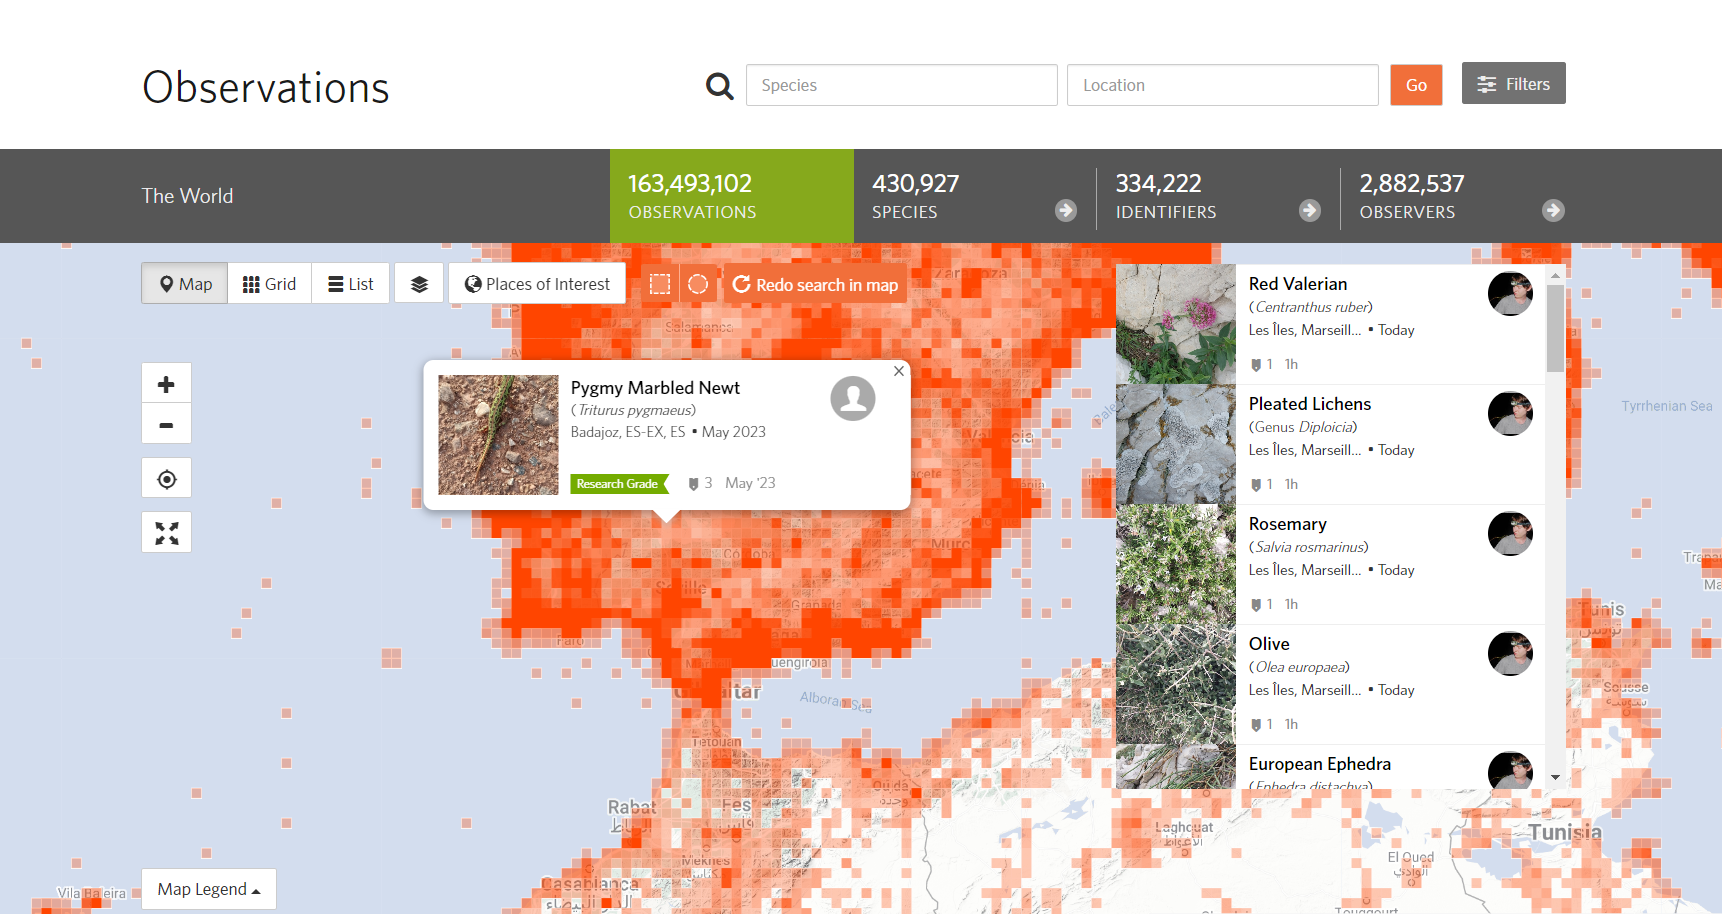
\includegraphics[width=\textwidth]{slike/inaturalist.PNG} %veličina u odnosu na širinu linije
				\caption{iNaturalist}
				\label{fig:inaturalist} %label mora biti drugaciji za svaku sliku
			\end{figure}
			
			\item eBird: eBird je aplikacija razvijena od strane Cornell Lab of Ornithology, fokusirana na ptice. Korisnici mogu bilježiti svoja opažanja o pticama te pridonositi globalnoj bazi podataka o pticama.
			\begin{figure}[H]
				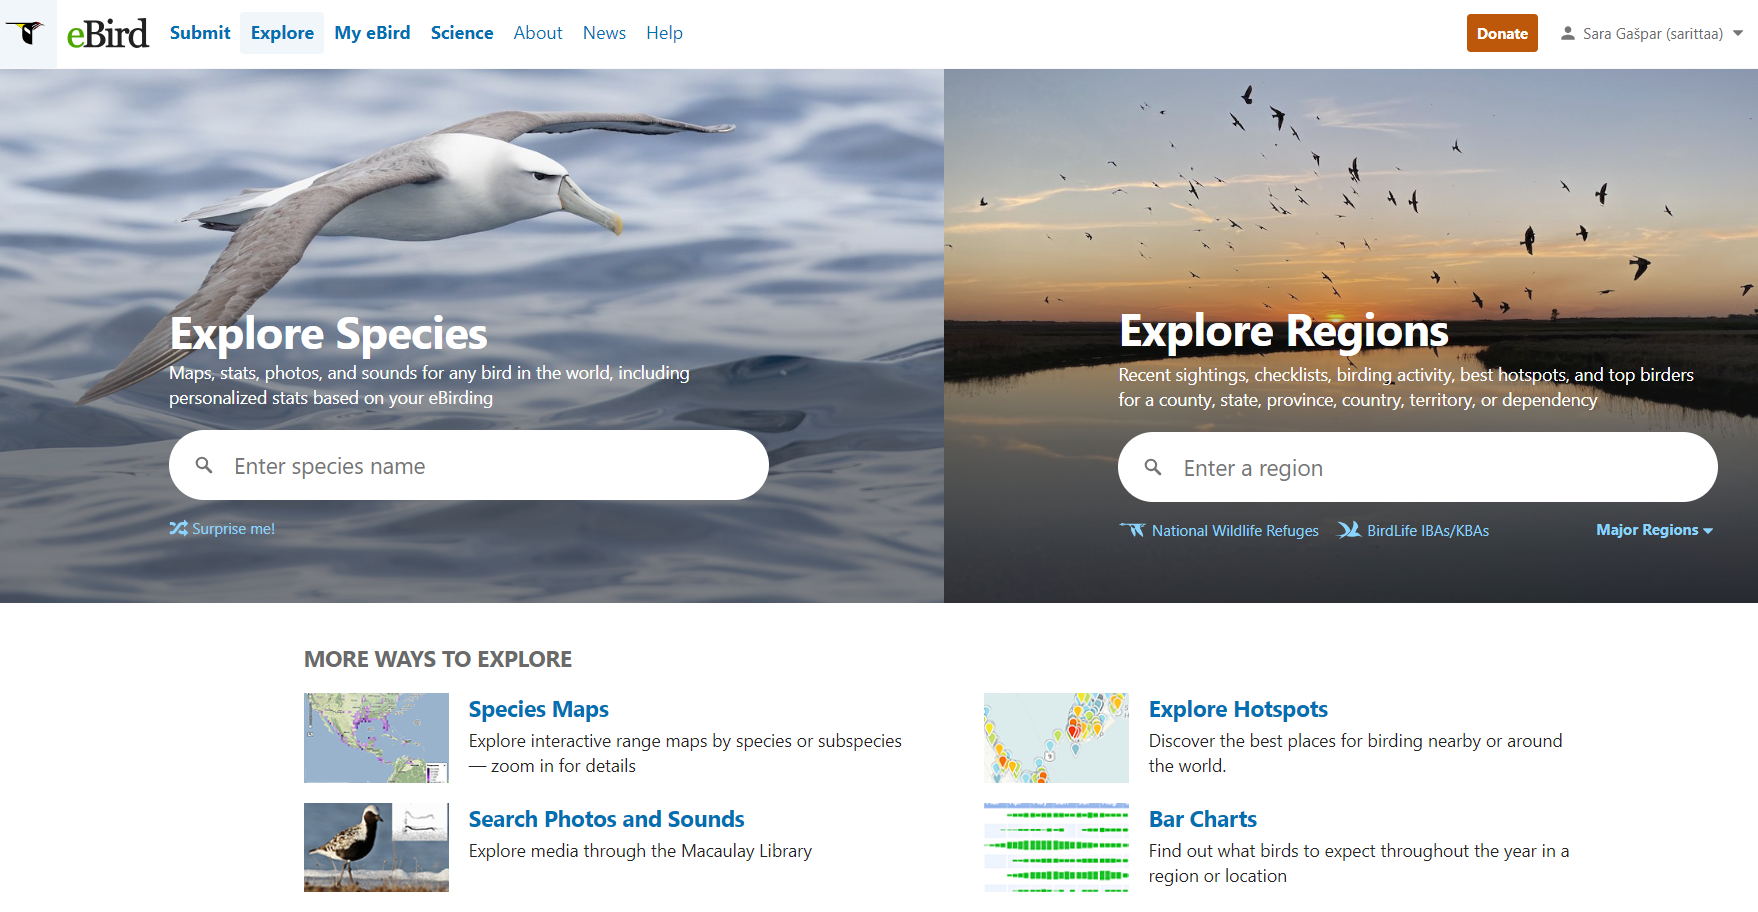
\includegraphics[width=\textwidth]{slike/ebird.PNG} %veličina u odnosu na širinu linije
				\caption{eBird}
				\label{fig:ebird} %label mora biti drugaciji za svaku sliku
			\end{figure}
			\item 
			
			Movebank: Ova platforma omogućuje istraživačima da prate ponašanje divljih životinja putem GPS uređaja, odašiljača i drugih senzora, te analiziraju ove podatke u stvarnom vremenu.
			\begin{figure}[H]
				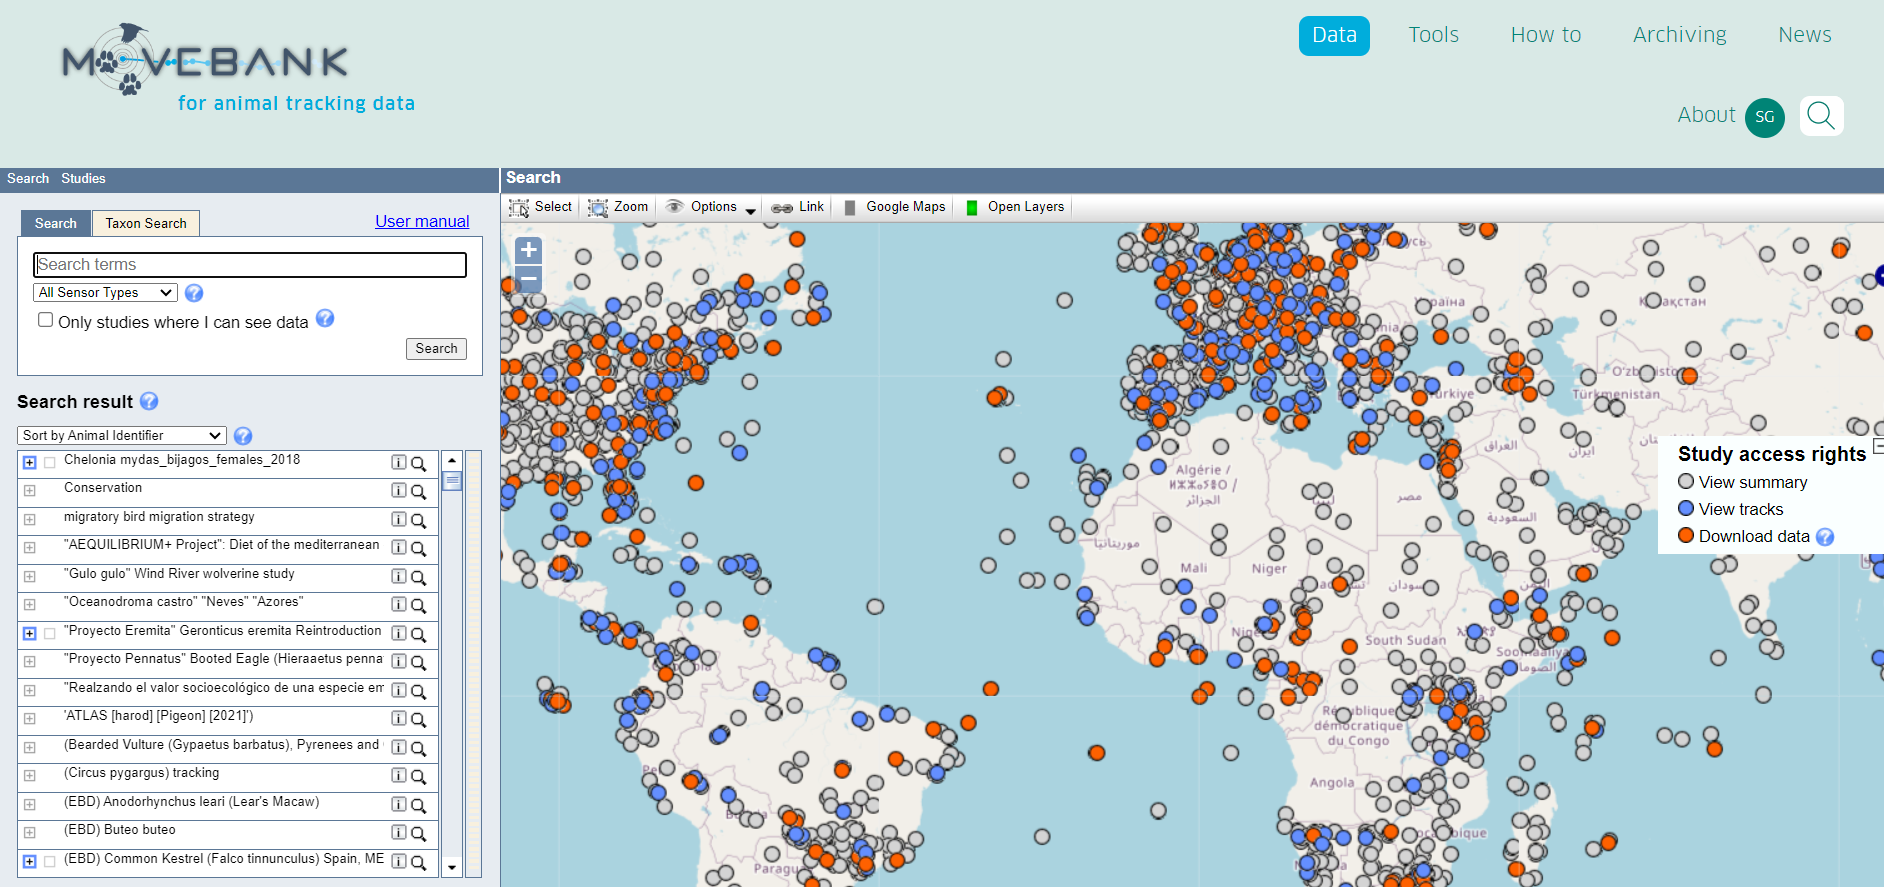
\includegraphics[width=\textwidth]{slike/movebank.PNG} %veličina u odnosu na širinu linije
				\caption{Movebank}
				\label{fig:movebank} %label mora biti drugaciji za svaku sliku
			\end{figure}
			\item Project Noah: Ova aplikacija omogućava korisnicima da dijele fotografije divljih životinja i biljaka te surađuju s globalnom zajednicom kako bi identificirali vrste.
			\begin{figure}[H]
				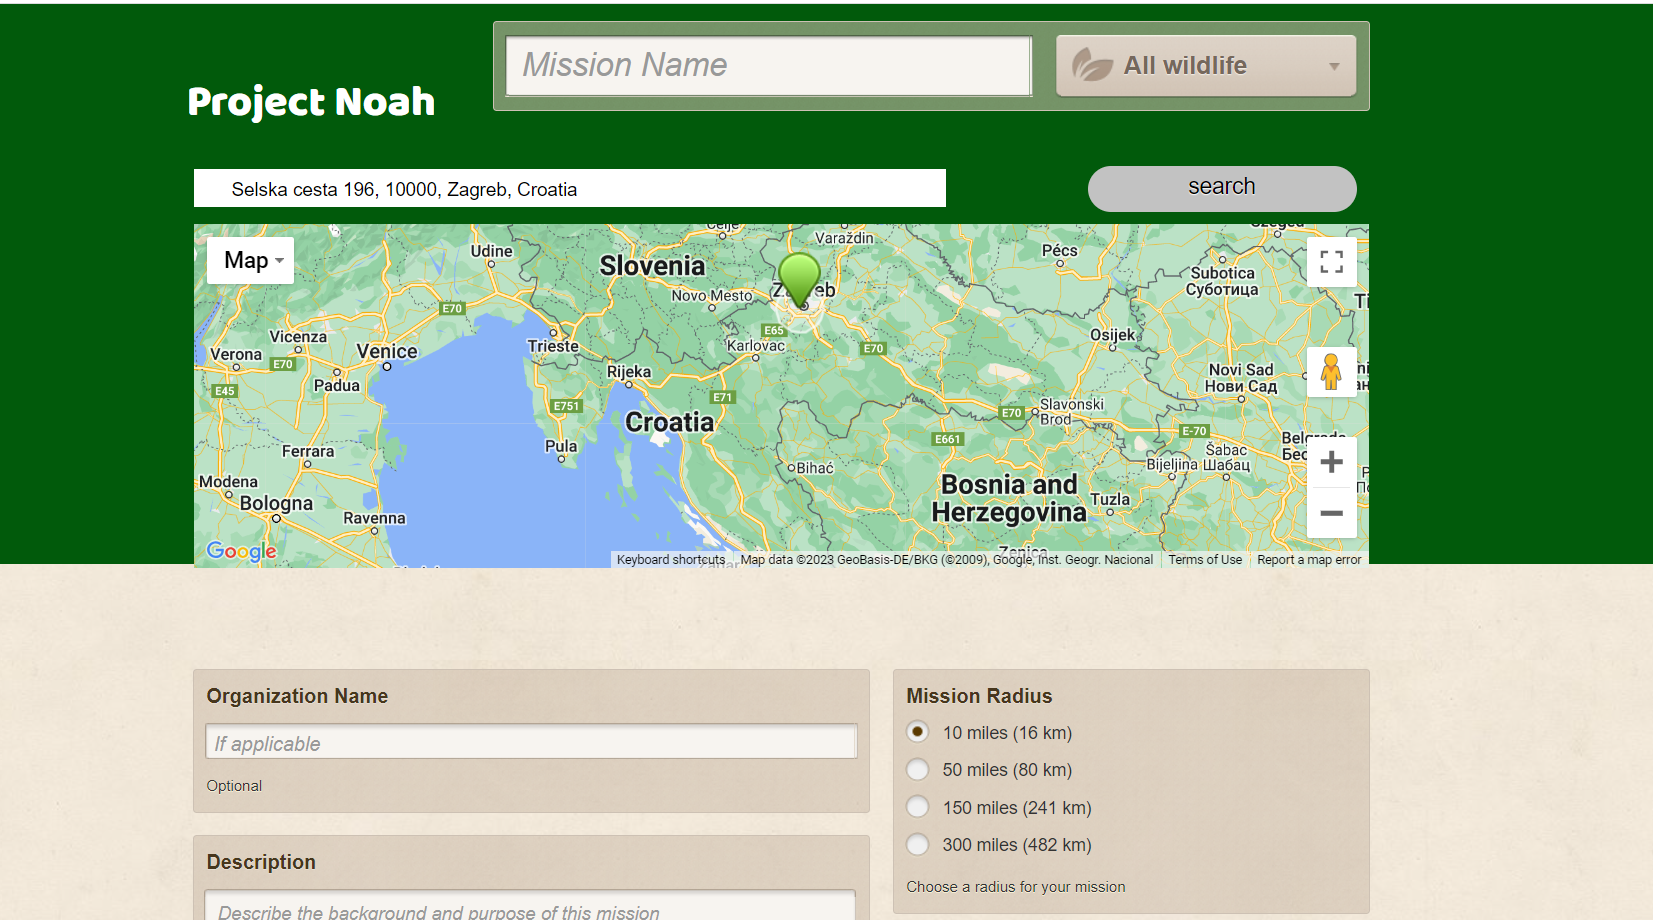
\includegraphics[width=\textwidth]{slike/projectnoah.PNG} %veličina u odnosu na širinu linije
				\caption{Project Noah}
				\label{fig:projectnoah} %label mora biti drugaciji za svaku sliku
			\end{figure}
			
		\end{packed_item}
		
		\vspace{36pt}
		
		Svaka od ovih aplikacija ima svoje specifične značajke i usmjerena je na različite vrste divljih životinja ili na različite vrste istraživanja. Wildtrack bi mogao kombinirati neke od ovih značajki, kreiranje akcija poput Project Noah-a te praćenje životinja poput Movebank-a pružajući jedinstvenu platformu koja omogućava suradnju između različitih korisničkih uloga i pruža specifične alate za istraživače, voditelje postaja i terenske tragače. U nastavku ćemo detaljnije istražiti ključne značajke i prednosti ove inovativne web aplikacije.\newline
		
		Prilikom pokretanja aplikacije, neregistriranom korisniku otvara se ekran na kojem ima dvije mogućnosti: prijaviti se u sustav već postojećim računom koristeći korisničko ime i lozinku ili stvoriti novi račun registracijom. Pri stvaranju novog računa, potrebno je unijeti sljedeće podatke: korisničko ime, fotografiju, lozinku, ime, prezime te email adresu. Registrirati se može kao jedan od tri različite vrste korisnika: voditelj postaje, istraživač te tragač. Registracija se završava potvrdom preko email adrese, a istraživača i voditelja postaje dodatno treba potvrditi administrator. Tek kada je korisnik registriran i prijavljen u sustav, može iskusiti sve funkcionalnosti naše web aplikacije.\newline
		
		Praćene životinje na sebi imaju GPS uređaj koji aplikaciji odašilje svoju poziciju. O praćenim životinjama se zapisuju povijesni podaci gdje se nalazila, naziv vrste, slika i opis. Korisnicima se te informacije prikazuju na karti. \newline
		
		U aplikaciji postoje četiri različite vrste korisnika: tragač, istražitelj, voditelj postaje, te administrator. Svaka od ovih uloga ima specifične zadatke i odgovornosti. Tragači koriste GPS uređaje za praćenje životinja i obavljanje zadataka koje im dodijele istraživači. Istraživači su kreatori akcija praćenja, određuju vrste i lokacije praćenja te dodjeljuju zadatke tragačima. Voditelji postaje su odgovorni za određeno geografsko područje i organizaciju tragača unutar svoje postaje. U nastavku ćemo opisati mogućnosti i ovlasti svake od vrsta korisnika. \newline
		
		\textbf{Voditelj} postaje ima mogućnost na karti odabrati jednu od ponuđenih postaja koja obuhvaća određeni prostor i ima svoje ime, npr. postaja Lonjsko polje ili Biokovo. Kada je odabrao svoju postaju, ima mogućnost odabrati tragače svoje postaje. Osim toga, voditelj definira na koji način su njegovi tragači osposobljeni izvoditi pretraživanje. Mogu biti osposobljeni za izvođenje zadataka pješke, dronom, automobilom, cross motorom, brodom ili helikopterom. Svaka metoda pretraživanja pruža različitu vidljivost i područje pokrivanja te se na prikladan način prikazuje na karti. Voditelj također može vidjeti prikaz karte sa svojim tragačima. \newline
		
		\textbf{Istraživač} je zadužen za kreiranje novih akcija pretraživanja i praćenja s detaljima o određenim vrstama, jedinkama ili staništima za proučavanje. Svaki istraživač zadužen je samo za jednu akciju. Prilikom stvaranja akcije, istraživač voditelju stanice šalje zahtjev za tragačima. U zahtjevu treba napisati broj ljudi koji mu je potreban za akciju, te zadatke koje je potrebno obaviti. Svaka akcija ima jednog istraživača i više tragača, a odnosi se na postaju jednog ili više voditelja. Ako mu voditelj ili voditelji odobre zahtjev (imaju dovoljan broj kvalificiranih ljudi) šalju mu popis dodijeljenih tragača i tada im istraživač mora pojedinačno podijeliti konkretne zadatke. Zadatak može biti prolazak određenom rutom, dolazak do lokacije, postavljanje kamere, te postavljanje GPS uređaja za praćenje na životinje.  U slučaju da voditelj u trenutku slanja zahtjeva nema dovoljan broj odgovarajućih tragača, istraživaču će zahtjev biti odbijen, te ima mogućnost poslati novi. Istraživaču se na njegovom početnom ekranu prikazuje interaktivna karta s informacijama o pozicijama životinja, tragača i postaja. Istraživač može odabrati da se za izradu karata koriste neka od idućih informacija: povijesne pozicije svih praćenih životinja, filtrirano po vrsti ili pojedinačno po jedinki te trenutne pozicije praćenih životinja; povijesne pozicije svih tragača na nekoj akciji, filtrirano po tipu prijevoza ili pojedinačno po tragaču te trenutne pozicije tragača aktivnih na akciji. \newline
		
		\textbf{Tragač} ima ulogu praćenja životinja i obavljanja zadataka koje mu je dodijelio istraživač. Njegov početni ekran nakon prijave u sustav sadrži kartu na kojoj su mu prikazani zadaci koje treba obaviti, trenutna pozicija ostalih tragača aktivnih na istoj akciji, te trenutna pozicija praćenih životinja. Tragač na jednoj akciji ne mijenja tip prijevoza. Tragač se može maknuti s akcije završetkom svih potrebnih zadataka, a staze kojima prolazi zapisuju se u bazu. \newline
		
		\textbf{Administrator} je uloga s najvećim ovlastima i ima ju samo jedna osoba. Administrator mora potvrditi registraciju ukoliko se radi o istraživačima i voditeljima postaja. Osim toga, administrator može vidjeti popis svih registriranih korisnika i njihovih osobnih podataka te im mijenjati dodijeljena prava i osobne podatke. \newline
		
		Wildtrack također pruža mogućnost suradnje među korisnicima putem komentara i povratnih informacija. Tragači mogu ostavljati komentare o praćenju životinja, dijeliti svoja iskustva i surađivati u stvarnom vremenu. Istraživači mogu pratiti napredak svojih akcija, analizirati podatke koje prikupljaju tragači te prilagoditi strategije praćenja. Svaka akcija praćenja životinja u Wildtrack aplikaciji pridonosi bazi podataka o divljim životinjama. Ovi podaci služe istraživačima i znanstvenicima za dublje razumijevanje migracija, ponašanja i ekologije različitih vrsta. Wildtrack je više od aplikacije - to je platforma koja potiče zajednički rad i edukaciju o važnosti divljih životinja u našem ekosustavu. Ova inicijativa ima potencijal potaknuti globalnu suradnju u zaštiti prirode i očuvanju biološke raznolikosti našeg planeta. \newline
		
		
		
		
	
	\chapter{Specifikacija programske potpore}
		
	\section{Funkcionalni zahtjevi}
			
			\textbf{\textit{dio 1. revizije}}\\
			
			\textit{Navesti \textbf{dionike} koji imaju \textbf{interes u ovom sustavu} ili  \textbf{su nositelji odgovornosti}. To su prije svega korisnici, ali i administratori sustava, naručitelji, razvojni tim.}\\
				
			\textit{Navesti \textbf{aktore} koji izravno \textbf{koriste} ili \textbf{komuniciraju sa sustavom}. Oni mogu imati inicijatorsku ulogu, tj. započinju određene procese u sustavu ili samo sudioničku ulogu, tj. obavljaju određeni posao. Za svakog aktora navesti funkcionalne zahtjeve koji se na njega odnose.}\\
			
			
			\noindent \textbf{Dionici:}
			
			\begin{packed_enum}
				
				\item Voditelj postaje
				\item Istraživač	
				\item Tragač
				\item Administrator
				
			\end{packed_enum}
			
			\noindent \textbf{Aktori i njihovi funkcionalni zahtjevi:}
			
			
			\begin{packed_enum}
				\item  \underbar{Voditelj postaje može:}
				
				\begin{packed_enum}
					
					\item vidjeti kartu s ponuđenim postajama
					\item odabrati postaju čiji voditelj želi postati
					\item odabrati tragače svoje postaje
					\item definirati način prijevoza svojih tragača - pješke, dronom, automobilom, cross motorom, brodom ili helikopterom
					\item prihvatiti ili odbiti zahtjev za tragačima od istraživača
					
				\end{packed_enum}
			
				\item  \underbar{Istraživač može:}
				
				\begin{packed_enum}
					
					\item kreirati nove akcije pretraživanja i praćenja životinja
					\item poslati zahtjev za tragačima voditelju postaje
					\item podijeliti zadatke tragačima koje je dobio od voditelja postaje
					\item vidjeti interaktivnu kartu s podacima o pozicijama životinja, životinja, tragača i postaja
					\item odabrati kriterije filtriranja karte
					
				\end{packed_enum}
				
				\item  \underbar{Tragač može:}
				
				\begin{packed_enum}
					
					\item na karti vidjeti svoje zadatke, životinje te ostale tragače na istoj akciji
					\item Obavljati zadatke koje mu je dodijelio istraživač
					\item Prilikom obavljanja akcije ostaviti komentar za ostale tragače
					
				\end{packed_enum}
				
				
			\end{packed_enum}
			
			\eject 
			
			
				
			\subsection{Obrasci uporabe}
				
				\textbf{\textit{dio 1. revizije}}
				
				\subsubsection{Opis obrazaca uporabe}
					\textit{Funkcionalne zahtjeve razraditi u obliku obrazaca uporabe. Svaki obrazac je potrebno razraditi prema donjem predlošku. Ukoliko u nekom koraku može doći do odstupanja, potrebno je to odstupanje opisati i po mogućnosti ponuditi rješenje kojim bi se tijek obrasca vratio na osnovni tijek.}\\
					

					\noindent \underbar{\textbf{UC1 - Registracija}}
					\begin{packed_item}
	
						\item \textbf{Glavni sudionik: }$<$sudionik$>$
						\item  \textbf{Cilj:} $<$cilj$>$
						\item  \textbf{Sudionici:} $<$sudionici$>$
						\item  \textbf{Preduvjet:} $<$preduvjet$>$
						\item  \textbf{Opis osnovnog tijeka:}
						
						\item[] \begin{packed_enum}
	
							\item $<$opis korak jedan$>$
							\item $<$opis korak dva$>$
							\item $<$opis korak tri$>$
							\item $<$opis korak četiri$>$
							\item $<$opis korak pet$>$
						\end{packed_enum}
						
						\item  \textbf{Opis mogućih odstupanja:}
						
						\item[] \begin{packed_item}
	
							\item[2.a] $<$opis mogućeg scenarija odstupanja u koraku 2$>$
							\item[] \begin{packed_enum}
								
								\item $<$opis rješenja mogućeg scenarija korak 1$>$
								\item $<$opis rješenja mogućeg scenarija korak 2$>$
								
							\end{packed_enum}
							\item[2.b] $<$opis mogućeg scenarija odstupanja u koraku 2$>$
							\item[3.a] $<$opis mogućeg scenarija odstupanja  u koraku 3$>$
							
						\end{packed_item}
					\end{packed_item}
					
					\noindent \underbar{\textbf{UC2 - Prijava u sustav}}
					\begin{packed_item}
						
						\item \textbf{Glavni sudionik: }$<$sudionik$>$
						\item  \textbf{Cilj:} $<$cilj$>$
						\item  \textbf{Sudionici:} $<$sudionici$>$
						\item  \textbf{Preduvjet:} $<$preduvjet$>$
						\item  \textbf{Opis osnovnog tijeka:}
						
						\item[] \begin{packed_enum}
							
							\item $<$opis korak jedan$>$
							\item $<$opis korak dva$>$
							\item $<$opis korak tri$>$
							\item $<$opis korak četiri$>$
							\item $<$opis korak pet$>$
						\end{packed_enum}
						
						\item  \textbf{Opis mogućih odstupanja:}
						
						\item[] \begin{packed_item}
							
							\item[2.a] $<$opis mogućeg scenarija odstupanja u koraku 2$>$
							\item[] \begin{packed_enum}
								
								\item $<$opis rješenja mogućeg scenarija korak 1$>$
								\item $<$opis rješenja mogućeg scenarija korak 2$>$
								
							\end{packed_enum}
							\item[2.b] $<$opis mogućeg scenarija odstupanja u koraku 2$>$
							\item[3.a] $<$opis mogućeg scenarija odstupanja  u koraku 3$>$
							
						\end{packed_item}
					\end{packed_item}
					
					\noindent \underbar{\textbf{UC3 - Pregled osobnih podataka}}
					\begin{packed_item}
						
						\item \textbf{Glavni sudionik: }$<$sudionik$>$
						\item  \textbf{Cilj:} $<$cilj$>$
						\item  \textbf{Sudionici:} $<$sudionici$>$
						\item  \textbf{Preduvjet:} $<$preduvjet$>$
						\item  \textbf{Opis osnovnog tijeka:}
						
						\item[] \begin{packed_enum}
							
							\item $<$opis korak jedan$>$
							\item $<$opis korak dva$>$
							\item $<$opis korak tri$>$
							\item $<$opis korak četiri$>$
							\item $<$opis korak pet$>$
						\end{packed_enum}
						
						\item  \textbf{Opis mogućih odstupanja:}
						
						\item[] \begin{packed_item}
							
							\item[2.a] $<$opis mogućeg scenarija odstupanja u koraku 2$>$
							\item[] \begin{packed_enum}
								
								\item $<$opis rješenja mogućeg scenarija korak 1$>$
								\item $<$opis rješenja mogućeg scenarija korak 2$>$
								
							\end{packed_enum}
							\item[2.b] $<$opis mogućeg scenarija odstupanja u koraku 2$>$
							\item[3.a] $<$opis mogućeg scenarija odstupanja  u koraku 3$>$
							
						\end{packed_item}
					\end{packed_item}
					
					\noindent \underbar{\textbf{UC4 - Promjena osobnih podataka}}
					\begin{packed_item}
						
						\item \textbf{Glavni sudionik: }$<$sudionik$>$
						\item  \textbf{Cilj:} $<$cilj$>$
						\item  \textbf{Sudionici:} $<$sudionici$>$
						\item  \textbf{Preduvjet:} $<$preduvjet$>$
						\item  \textbf{Opis osnovnog tijeka:}
						
						\item[] \begin{packed_enum}
							
							\item $<$opis korak jedan$>$
							\item $<$opis korak dva$>$
							\item $<$opis korak tri$>$
							\item $<$opis korak četiri$>$
							\item $<$opis korak pet$>$
						\end{packed_enum}
						
						\item  \textbf{Opis mogućih odstupanja:}
						
						\item[] \begin{packed_item}
							
							\item[2.a] $<$opis mogućeg scenarija odstupanja u koraku 2$>$
							\item[] \begin{packed_enum}
								
								\item $<$opis rješenja mogućeg scenarija korak 1$>$
								\item $<$opis rješenja mogućeg scenarija korak 2$>$
								
							\end{packed_enum}
							\item[2.b] $<$opis mogućeg scenarija odstupanja u koraku 2$>$
							\item[3.a] $<$opis mogućeg scenarija odstupanja  u koraku 3$>$
							
						\end{packed_item}
					\end{packed_item}
					
					\noindent \underbar{\textbf{UC5 - Brisanje korisničkog računa}}
					\begin{packed_item}
						
						\item \textbf{Glavni sudionik: }$<$sudionik$>$
						\item  \textbf{Cilj:} $<$cilj$>$
						\item  \textbf{Sudionici:} $<$sudionici$>$
						\item  \textbf{Preduvjet:} $<$preduvjet$>$
						\item  \textbf{Opis osnovnog tijeka:}
						
						\item[] \begin{packed_enum}
							
							\item $<$opis korak jedan$>$
							\item $<$opis korak dva$>$
							\item $<$opis korak tri$>$
							\item $<$opis korak četiri$>$
							\item $<$opis korak pet$>$
						\end{packed_enum}
						
						\item  \textbf{Opis mogućih odstupanja:}
						
						\item[] \begin{packed_item}
							
							\item[2.a] $<$opis mogućeg scenarija odstupanja u koraku 2$>$
							\item[] \begin{packed_enum}
								
								\item $<$opis rješenja mogućeg scenarija korak 1$>$
								\item $<$opis rješenja mogućeg scenarija korak 2$>$
								
							\end{packed_enum}
							\item[2.b] $<$opis mogućeg scenarija odstupanja u koraku 2$>$
							\item[3.a] $<$opis mogućeg scenarija odstupanja  u koraku 3$>$
							
						\end{packed_item}
					\end{packed_item}
					
					\noindent \underbar{\textbf{UC6 - Potvrda korisnika mailom}}
					\begin{packed_item}
						
						\item \textbf{Glavni sudionik: }$<$sudionik$>$
						\item  \textbf{Cilj:} $<$cilj$>$
						\item  \textbf{Sudionici:} $<$sudionici$>$
						\item  \textbf{Preduvjet:} $<$preduvjet$>$
						\item  \textbf{Opis osnovnog tijeka:}
						
						\item[] \begin{packed_enum}
							
							\item $<$opis korak jedan$>$
							\item $<$opis korak dva$>$
							\item $<$opis korak tri$>$
							\item $<$opis korak četiri$>$
							\item $<$opis korak pet$>$
						\end{packed_enum}
						
						\item  \textbf{Opis mogućih odstupanja:}
						
						\item[] \begin{packed_item}
							
							\item[2.a] $<$opis mogućeg scenarija odstupanja u koraku 2$>$
							\item[] \begin{packed_enum}
								
								\item $<$opis rješenja mogućeg scenarija korak 1$>$
								\item $<$opis rješenja mogućeg scenarija korak 2$>$
								
							\end{packed_enum}
							\item[2.b] $<$opis mogućeg scenarija odstupanja u koraku 2$>$
							\item[3.a] $<$opis mogućeg scenarija odstupanja  u koraku 3$>$
							
						\end{packed_item}
					\end{packed_item}
					
					\noindent \underbar{\textbf{UC7 - Potvrda uloge od strane admina}}
					\begin{packed_item}
						
						\item \textbf{Glavni sudionik: }$<$sudionik$>$
						\item  \textbf{Cilj:} $<$cilj$>$
						\item  \textbf{Sudionici:} $<$sudionici$>$
						\item  \textbf{Preduvjet:} $<$preduvjet$>$
						\item  \textbf{Opis osnovnog tijeka:}
						
						\item[] \begin{packed_enum}
							
							\item $<$opis korak jedan$>$
							\item $<$opis korak dva$>$
							\item $<$opis korak tri$>$
							\item $<$opis korak četiri$>$
							\item $<$opis korak pet$>$
						\end{packed_enum}
						
						\item  \textbf{Opis mogućih odstupanja:}
						
						\item[] \begin{packed_item}
							
							\item[2.a] $<$opis mogućeg scenarija odstupanja u koraku 2$>$
							\item[] \begin{packed_enum}
								
								\item $<$opis rješenja mogućeg scenarija korak 1$>$
								\item $<$opis rješenja mogućeg scenarija korak 2$>$
								
							\end{packed_enum}
							\item[2.b] $<$opis mogućeg scenarija odstupanja u koraku 2$>$
							\item[3.a] $<$opis mogućeg scenarija odstupanja  u koraku 3$>$
							
						\end{packed_item}
					\end{packed_item}
					
					\noindent \underbar{\textbf{UC8 - Prikazivanje pozicije životinje}}
					\begin{packed_item}
						
						\item \textbf{Glavni sudionik: }$<$sudionik$>$
						\item  \textbf{Cilj:} $<$cilj$>$
						\item  \textbf{Sudionici:} $<$sudionici$>$
						\item  \textbf{Preduvjet:} $<$preduvjet$>$
						\item  \textbf{Opis osnovnog tijeka:}
						
						\item[] \begin{packed_enum}
							
							\item $<$opis korak jedan$>$
							\item $<$opis korak dva$>$
							\item $<$opis korak tri$>$
							\item $<$opis korak četiri$>$
							\item $<$opis korak pet$>$
						\end{packed_enum}
						
						\item  \textbf{Opis mogućih odstupanja:}
						
						\item[] \begin{packed_item}
							
							\item[2.a] $<$opis mogućeg scenarija odstupanja u koraku 2$>$
							\item[] \begin{packed_enum}
								
								\item $<$opis rješenja mogućeg scenarija korak 1$>$
								\item $<$opis rješenja mogućeg scenarija korak 2$>$
								
							\end{packed_enum}
							\item[2.b] $<$opis mogućeg scenarija odstupanja u koraku 2$>$
							\item[3.a] $<$opis mogućeg scenarija odstupanja  u koraku 3$>$
							
						\end{packed_item}
					\end{packed_item}
					
					\noindent \underbar{\textbf{UC9 - Prikazivanje pozicije tragača}}
					\begin{packed_item}
						
						\item \textbf{Glavni sudionik: }$<$sudionik$>$
						\item  \textbf{Cilj:} $<$cilj$>$
						\item  \textbf{Sudionici:} $<$sudionici$>$
						\item  \textbf{Preduvjet:} $<$preduvjet$>$
						\item  \textbf{Opis osnovnog tijeka:}
						
						\item[] \begin{packed_enum}
							
							\item $<$opis korak jedan$>$
							\item $<$opis korak dva$>$
							\item $<$opis korak tri$>$
							\item $<$opis korak četiri$>$
							\item $<$opis korak pet$>$
						\end{packed_enum}
						
						\item  \textbf{Opis mogućih odstupanja:}
						
						\item[] \begin{packed_item}
							
							\item[2.a] $<$opis mogućeg scenarija odstupanja u koraku 2$>$
							\item[] \begin{packed_enum}
								
								\item $<$opis rješenja mogućeg scenarija korak 1$>$
								\item $<$opis rješenja mogućeg scenarija korak 2$>$
								
							\end{packed_enum}
							\item[2.b] $<$opis mogućeg scenarija odstupanja u koraku 2$>$
							\item[3.a] $<$opis mogućeg scenarija odstupanja  u koraku 3$>$
							
						\end{packed_item}
					\end{packed_item}
					
					\noindent \underbar{\textbf{UC10 - Prikazivanje pozicije postaje}}
					\begin{packed_item}
						
						\item \textbf{Glavni sudionik: }$<$sudionik$>$
						\item  \textbf{Cilj:} $<$cilj$>$
						\item  \textbf{Sudionici:} $<$sudionici$>$
						\item  \textbf{Preduvjet:} $<$preduvjet$>$
						\item  \textbf{Opis osnovnog tijeka:}
						
						\item[] \begin{packed_enum}
							
							\item $<$opis korak jedan$>$
							\item $<$opis korak dva$>$
							\item $<$opis korak tri$>$
							\item $<$opis korak četiri$>$
							\item $<$opis korak pet$>$
						\end{packed_enum}
						
						\item  \textbf{Opis mogućih odstupanja:}
						
						\item[] \begin{packed_item}
							
							\item[2.a] $<$opis mogućeg scenarija odstupanja u koraku 2$>$
							\item[] \begin{packed_enum}
								
								\item $<$opis rješenja mogućeg scenarija korak 1$>$
								\item $<$opis rješenja mogućeg scenarija korak 2$>$
								
							\end{packed_enum}
							\item[2.b] $<$opis mogućeg scenarija odstupanja u koraku 2$>$
							\item[3.a] $<$opis mogućeg scenarija odstupanja  u koraku 3$>$
							
						\end{packed_item}
					\end{packed_item}
					
					\noindent \underbar{\textbf{UC11 - Prikaz informacija o životinji}}
					\begin{packed_item}
						
						\item \textbf{Glavni sudionik: }$<$sudionik$>$
						\item  \textbf{Cilj:} $<$cilj$>$
						\item  \textbf{Sudionici:} $<$sudionici$>$
						\item  \textbf{Preduvjet:} $<$preduvjet$>$
						\item  \textbf{Opis osnovnog tijeka:}
						
						\item[] \begin{packed_enum}
							
							\item $<$opis korak jedan$>$
							\item $<$opis korak dva$>$
							\item $<$opis korak tri$>$
							\item $<$opis korak četiri$>$
							\item $<$opis korak pet$>$
						\end{packed_enum}
						
						\item  \textbf{Opis mogućih odstupanja:}
						
						\item[] \begin{packed_item}
							
							\item[2.a] $<$opis mogućeg scenarija odstupanja u koraku 2$>$
							\item[] \begin{packed_enum}
								
								\item $<$opis rješenja mogućeg scenarija korak 1$>$
								\item $<$opis rješenja mogućeg scenarija korak 2$>$
								
							\end{packed_enum}
							\item[2.b] $<$opis mogućeg scenarija odstupanja u koraku 2$>$
							\item[3.a] $<$opis mogućeg scenarija odstupanja  u koraku 3$>$
							
						\end{packed_item}
					\end{packed_item}
					
					\noindent \underbar{\textbf{UC12 - Odabir postaje}}
					\begin{packed_item}
						
						\item \textbf{Glavni sudionik: }$<$sudionik$>$
						\item  \textbf{Cilj:} $<$cilj$>$
						\item  \textbf{Sudionici:} $<$sudionici$>$
						\item  \textbf{Preduvjet:} $<$preduvjet$>$
						\item  \textbf{Opis osnovnog tijeka:}
						
						\item[] \begin{packed_enum}
							
							\item $<$opis korak jedan$>$
							\item $<$opis korak dva$>$
							\item $<$opis korak tri$>$
							\item $<$opis korak četiri$>$
							\item $<$opis korak pet$>$
						\end{packed_enum}
						
						\item  \textbf{Opis mogućih odstupanja:}
						
						\item[] \begin{packed_item}
							
							\item[2.a] $<$opis mogućeg scenarija odstupanja u koraku 2$>$
							\item[] \begin{packed_enum}
								
								\item $<$opis rješenja mogućeg scenarija korak 1$>$
								\item $<$opis rješenja mogućeg scenarija korak 2$>$
								
							\end{packed_enum}
							\item[2.b] $<$opis mogućeg scenarija odstupanja u koraku 2$>$
							\item[3.a] $<$opis mogućeg scenarija odstupanja  u koraku 3$>$
							
						\end{packed_item}
					\end{packed_item}
					
					\noindent \underbar{\textbf{UC13 - Odabir tragača i definiranje kompetencija tragača}}
					\begin{packed_item}
						
						\item \textbf{Glavni sudionik: }$<$sudionik$>$
						\item  \textbf{Cilj:} $<$cilj$>$
						\item  \textbf{Sudionici:} $<$sudionici$>$
						\item  \textbf{Preduvjet:} $<$preduvjet$>$
						\item  \textbf{Opis osnovnog tijeka:}
						
						\item[] \begin{packed_enum}
							
							\item $<$opis korak jedan$>$
							\item $<$opis korak dva$>$
							\item $<$opis korak tri$>$
							\item $<$opis korak četiri$>$
							\item $<$opis korak pet$>$
						\end{packed_enum}
						
						\item  \textbf{Opis mogućih odstupanja:}
						
						\item[] \begin{packed_item}
							
							\item[2.a] $<$opis mogućeg scenarija odstupanja u koraku 2$>$
							\item[] \begin{packed_enum}
								
								\item $<$opis rješenja mogućeg scenarija korak 1$>$
								\item $<$opis rješenja mogućeg scenarija korak 2$>$
								
							\end{packed_enum}
							\item[2.b] $<$opis mogućeg scenarija odstupanja u koraku 2$>$
							\item[3.a] $<$opis mogućeg scenarija odstupanja  u koraku 3$>$
							
						\end{packed_item}
					\end{packed_item}
					
					\noindent \underbar{\textbf{UC14 - Uređivanje kompetencija tragača}}
					\begin{packed_item}
						
						\item \textbf{Glavni sudionik:} Voditelj
						\item  \textbf{Cilj:} Dodavanje ili brisanje kompetencija tragača 
						\item  \textbf{Sudionici:} Baza podataka, tragač
						\item  \textbf{Preduvjet:} Tragač je dio voditeljeve postaje
						\item  \textbf{Opis osnovnog tijeka:}
						
						\item[] \begin{packed_enum}
							
							\item Voditelj odabire jednog tragača
							\item Voditelj dodaje nove ili briše postojeće kompetencije odabranog tragača
							\item Unešene promjene se spremaju u bazu podataka
							\item Voditelju i tragaču se prikazuju ažurirane kompetencije
						\end{packed_enum}
					\end{packed_item}
					
					\noindent \underbar{\textbf{UC15 - Brisanje tragača}}
					\begin{packed_item}
						
						\item \textbf{Glavni sudionik: }Voditelj
						\item  \textbf{Cilj:} Trajno brisanje tragača iz postaje
						\item  \textbf{Sudionici:} Baza podataka,voditelj
						\item  \textbf{Preduvjet:} Tragač je dio voditeljeve postaje
						\item  \textbf{Opis osnovnog tijeka:}
						
						\item[] \begin{packed_enum}
							
							\item Voditelj odabire određenog tragača
							\item Voditelj ga briše iz svoje postaje
							\item Unešena promjena se sprema u bazu podataka
							\item Tragač dobiva informaciju o voditeljevoj odluci
						\end{packed_enum}
					\end{packed_item}
					
					\noindent \underbar{\textbf{UC16 - Pregled popisa tragača}}
					\begin{packed_item}
						
						\item \textbf{Glavni sudionik: }Voditelj
						\item  \textbf{Cilj:} Voditeljev pregled svih tragača
						\item  \textbf{Sudionici:} Baza podataka,voditelj
						\item  \textbf{Preduvjet:} Tragač je dio voditeljeve postaje
						\item  \textbf{Opis osnovnog tijeka:}
						
						\item[] \begin{packed_enum}
							
							\item Voditelj odabire tragače svoje postaje
							\item Voditelju se prikaže popis njegovih tragača
							\item Unešene promjene spremaju se u bazu podataka
						\end{packed_enum}
					\end{packed_item}
					
					\noindent \underbar{\textbf{UC17 - Pregled zahtjeva}}
					\begin{packed_item}
						
						\item \textbf{Glavni sudionik: }Voditelj
						\item  \textbf{Cilj:} Započeti komunikaciju između voditelja i istraživača 
						\item  \textbf{Sudionici:} Voditelj,istraživač
						\item  \textbf{Preduvjet:} -
						\item  \textbf{Opis osnovnog tijeka:}
						
						\item[] \begin{packed_enum}
							
							\item Istraživač voditelju šalje zahtjev za tragačima
							\item U zahtjevu zapisan broj potrebnih ljudi i zadaci
							\item Voditelj dobiva zahtjev te dalje slijedi obrada
						\end{packed_enum}
					\end{packed_item}
					
					\noindent \underbar{\textbf{UC18 - Obrada zahtjeva}}
					\begin{packed_item}
						
						\item \textbf{Glavni sudionik: }Voditelj
						\item  \textbf{Cilj:} Odobriti ili odbiti zahtjev
						\item  \textbf{Sudionici:} Voditelj
						\item  \textbf{Preduvjet:} Istraživač prethodno poslao zahtjev
						\item  \textbf{Opis osnovnog tijeka:}
						
						\item[] \begin{packed_enum}

							\item Istraživač poslao zahtjev							
							\item Zahtjev stigao do voditelja
							\item Voditelj donosi odluku na temelju broja dostupnih kvalificiranih ljudi
							\item Voditelj šalje odgovor na zahtjev istraživaču
							
						\end{packed_enum}
					\end{packed_item}
					
					\noindent \underbar{\textbf{UC19 - Kreiranje akcije}}
					\begin{packed_item}
						
						\item \textbf{Glavni sudionik: }$<$sudionik$>$
						\item  \textbf{Cilj:} $<$cilj$>$
						\item  \textbf{Sudionici:} $<$sudionici$>$
						\item  \textbf{Preduvjet:} $<$preduvjet$>$
						\item  \textbf{Opis osnovnog tijeka:}
						
						\item[] \begin{packed_enum}
							
							\item $<$opis korak jedan$>$
							\item $<$opis korak dva$>$
							\item $<$opis korak tri$>$
							\item $<$opis korak četiri$>$
							\item $<$opis korak pet$>$
						\end{packed_enum}
						
						\item  \textbf{Opis mogućih odstupanja:}
						
						\item[] \begin{packed_item}
							
							\item[2.a] $<$opis mogućeg scenarija odstupanja u koraku 2$>$
							\item[] \begin{packed_enum}
								
								\item $<$opis rješenja mogućeg scenarija korak 1$>$
								\item $<$opis rješenja mogućeg scenarija korak 2$>$
								
							\end{packed_enum}
							\item[2.b] $<$opis mogućeg scenarija odstupanja u koraku 2$>$
							\item[3.a] $<$opis mogućeg scenarija odstupanja  u koraku 3$>$
							
						\end{packed_item}
					\end{packed_item}
					
					\noindent \underbar{\textbf{UC20 - Slanje zahtjeva voditelju}}
					\begin{packed_item}
						
						\item \textbf{Glavni sudionik: }$<$sudionik$>$
						\item  \textbf{Cilj:} $<$cilj$>$
						\item  \textbf{Sudionici:} $<$sudionici$>$
						\item  \textbf{Preduvjet:} $<$preduvjet$>$
						\item  \textbf{Opis osnovnog tijeka:}
						
						\item[] \begin{packed_enum}
							
							\item $<$opis korak jedan$>$
							\item $<$opis korak dva$>$
							\item $<$opis korak tri$>$
							\item $<$opis korak četiri$>$
							\item $<$opis korak pet$>$
						\end{packed_enum}
						
						\item  \textbf{Opis mogućih odstupanja:}
						
						\item[] \begin{packed_item}
							
							\item[2.a] $<$opis mogućeg scenarija odstupanja u koraku 2$>$
							\item[] \begin{packed_enum}
								
								\item $<$opis rješenja mogućeg scenarija korak 1$>$
								\item $<$opis rješenja mogućeg scenarija korak 2$>$
								
							\end{packed_enum}
							\item[2.b] $<$opis mogućeg scenarija odstupanja u koraku 2$>$
							\item[3.a] $<$opis mogućeg scenarija odstupanja  u koraku 3$>$
							
						\end{packed_item}
					\end{packed_item}
					
					\noindent \underbar{\textbf{UC21 - Pregled stanja zahtjeva}}
					\begin{packed_item}
						
						\item \textbf{Glavni sudionik: }$<$sudionik$>$
						\item  \textbf{Cilj:} $<$cilj$>$
						\item  \textbf{Sudionici:} $<$sudionici$>$
						\item  \textbf{Preduvjet:} $<$preduvjet$>$
						\item  \textbf{Opis osnovnog tijeka:}
						
						\item[] \begin{packed_enum}
							
							\item $<$opis korak jedan$>$
							\item $<$opis korak dva$>$
							\item $<$opis korak tri$>$
							\item $<$opis korak četiri$>$
							\item $<$opis korak pet$>$
						\end{packed_enum}
						
						\item  \textbf{Opis mogućih odstupanja:}
						
						\item[] \begin{packed_item}
							
							\item[2.a] $<$opis mogućeg scenarija odstupanja u koraku 2$>$
							\item[] \begin{packed_enum}
								
								\item $<$opis rješenja mogućeg scenarija korak 1$>$
								\item $<$opis rješenja mogućeg scenarija korak 2$>$
								
							\end{packed_enum}
							\item[2.b] $<$opis mogućeg scenarija odstupanja u koraku 2$>$
							\item[3.a] $<$opis mogućeg scenarija odstupanja  u koraku 3$>$
							
						\end{packed_item}
					\end{packed_item}
					
					\noindent \underbar{\textbf{UC22 - Kreiranje zadataka}}
					\begin{packed_item}
						
						\item \textbf{Glavni sudionik: }$<$sudionik$>$
						\item  \textbf{Cilj:} $<$cilj$>$
						\item  \textbf{Sudionici:} $<$sudionici$>$
						\item  \textbf{Preduvjet:} $<$preduvjet$>$
						\item  \textbf{Opis osnovnog tijeka:}
						
						\item[] \begin{packed_enum}
							
							\item $<$opis korak jedan$>$
							\item $<$opis korak dva$>$
							\item $<$opis korak tri$>$
							\item $<$opis korak četiri$>$
							\item $<$opis korak pet$>$
						\end{packed_enum}
						
						\item  \textbf{Opis mogućih odstupanja:}
						
						\item[] \begin{packed_item}
							
							\item[2.a] $<$opis mogućeg scenarija odstupanja u koraku 2$>$
							\item[] \begin{packed_enum}
								
								\item $<$opis rješenja mogućeg scenarija korak 1$>$
								\item $<$opis rješenja mogućeg scenarija korak 2$>$
								
							\end{packed_enum}
							\item[2.b] $<$opis mogućeg scenarija odstupanja u koraku 2$>$
							\item[3.a] $<$opis mogućeg scenarija odstupanja  u koraku 3$>$
							
						\end{packed_item}
					\end{packed_item}
					
					\noindent \underbar{\textbf{UC23 - Dodjela zadataka}}
					\begin{packed_item}
						
						\item \textbf{Glavni sudionik: }$<$sudionik$>$
						\item  \textbf{Cilj:} $<$cilj$>$
						\item  \textbf{Sudionici:} $<$sudionici$>$
						\item  \textbf{Preduvjet:} $<$preduvjet$>$
						\item  \textbf{Opis osnovnog tijeka:}
						
						\item[] \begin{packed_enum}
							
							\item $<$opis korak jedan$>$
							\item $<$opis korak dva$>$
							\item $<$opis korak tri$>$
							\item $<$opis korak četiri$>$
							\item $<$opis korak pet$>$
						\end{packed_enum}
						
						\item  \textbf{Opis mogućih odstupanja:}
						
						\item[] \begin{packed_item}
							
							\item[2.a] $<$opis mogućeg scenarija odstupanja u koraku 2$>$
							\item[] \begin{packed_enum}
								
								\item $<$opis rješenja mogućeg scenarija korak 1$>$
								\item $<$opis rješenja mogućeg scenarija korak 2$>$
								
							\end{packed_enum}
							\item[2.b] $<$opis mogućeg scenarija odstupanja u koraku 2$>$
							\item[3.a] $<$opis mogućeg scenarija odstupanja  u koraku 3$>$
							
						\end{packed_item}
					\end{packed_item}
					
					\noindent \underbar{\textbf{UC24 - Definiranje prikaza na karti}}
					\begin{packed_item}
						
						\item \textbf{Glavni sudionik: }$<$sudionik$>$
						\item  \textbf{Cilj:} $<$cilj$>$
						\item  \textbf{Sudionici:} $<$sudionici$>$
						\item  \textbf{Preduvjet:} $<$preduvjet$>$
						\item  \textbf{Opis osnovnog tijeka:}
						
						\item[] \begin{packed_enum}
							
							\item $<$opis korak jedan$>$
							\item $<$opis korak dva$>$
							\item $<$opis korak tri$>$
							\item $<$opis korak četiri$>$
							\item $<$opis korak pet$>$
						\end{packed_enum}
						
						\item  \textbf{Opis mogućih odstupanja:}
						
						\item[] \begin{packed_item}
							
							\item[2.a] $<$opis mogućeg scenarija odstupanja u koraku 2$>$
							\item[] \begin{packed_enum}
								
								\item $<$opis rješenja mogućeg scenarija korak 1$>$
								\item $<$opis rješenja mogućeg scenarija korak 2$>$
								
							\end{packed_enum}
							\item[2.b] $<$opis mogućeg scenarija odstupanja u koraku 2$>$
							\item[3.a] $<$opis mogućeg scenarija odstupanja  u koraku 3$>$
							
						\end{packed_item}
					\end{packed_item}
					
					\noindent \underbar{\textbf{UC25 - Postavljanje komentara na karti}}
					\begin{packed_item}
						
						\item \textbf{Glavni sudionik: }$<$sudionik$>$
						\item  \textbf{Cilj:} $<$cilj$>$
						\item  \textbf{Sudionici:} $<$sudionici$>$
						\item  \textbf{Preduvjet:} $<$preduvjet$>$
						\item  \textbf{Opis osnovnog tijeka:}
						
						\item[] \begin{packed_enum}
							
							\item $<$opis korak jedan$>$
							\item $<$opis korak dva$>$
							\item $<$opis korak tri$>$
							\item $<$opis korak četiri$>$
							\item $<$opis korak pet$>$
						\end{packed_enum}
						
						\item  \textbf{Opis mogućih odstupanja:}
						
						\item[] \begin{packed_item}
							
							\item[2.a] $<$opis mogućeg scenarija odstupanja u koraku 2$>$
							\item[] \begin{packed_enum}
								
								\item $<$opis rješenja mogućeg scenarija korak 1$>$
								\item $<$opis rješenja mogućeg scenarija korak 2$>$
								
							\end{packed_enum}
							\item[2.b] $<$opis mogućeg scenarija odstupanja u koraku 2$>$
							\item[3.a] $<$opis mogućeg scenarija odstupanja  u koraku 3$>$
							
						\end{packed_item}
					\end{packed_item}
					
					\noindent \underbar{\textbf{UC26 - Pregled komentara}}
					\begin{packed_item}
						
						\item \textbf{Glavni sudionik: }$<$sudionik$>$
						\item  \textbf{Cilj:} $<$cilj$>$
						\item  \textbf{Sudionici:} $<$sudionici$>$
						\item  \textbf{Preduvjet:} $<$preduvjet$>$
						\item  \textbf{Opis osnovnog tijeka:}
						
						\item[] \begin{packed_enum}
							
							\item $<$opis korak jedan$>$
							\item $<$opis korak dva$>$
							\item $<$opis korak tri$>$
							\item $<$opis korak četiri$>$
							\item $<$opis korak pet$>$
						\end{packed_enum}
						
						\item  \textbf{Opis mogućih odstupanja:}
						
						\item[] \begin{packed_item}
							
							\item[2.a] $<$opis mogućeg scenarija odstupanja u koraku 2$>$
							\item[] \begin{packed_enum}
								
								\item $<$opis rješenja mogućeg scenarija korak 1$>$
								\item $<$opis rješenja mogućeg scenarija korak 2$>$
								
							\end{packed_enum}
							\item[2.b] $<$opis mogućeg scenarija odstupanja u koraku 2$>$
							\item[3.a] $<$opis mogućeg scenarija odstupanja  u koraku 3$>$
							
						\end{packed_item}
					\end{packed_item}
					
					\noindent \underbar{\textbf{UC27 - Brisanje komentara}}
					\begin{packed_item}
						
						\item \textbf{Glavni sudionik:} Istraživač, tragač
						\item  \textbf{Cilj:} Obrisati objavljeni komentar
						\item  \textbf{Sudionici:} Baza podataka
						\item  \textbf{Preduvjet:} Uloga istraživača ili tragača
						\item  \textbf{Opis osnovnog tijeka:}
						
						\item[] \begin{packed_enum}
							
							\item Glavni sudionik odabire svoj komentar
							\item Glavni sudionik odabire opciju "Obriši komentar"
							\item Komentar se briše iz baze podataka
							\item Komentar se više ne prikazuje istraživačima i tragačima
						\end{packed_enum}
					\end{packed_item}
					
					\noindent \underbar{\textbf{UC28 - Prikaz karte s tragačima na akciji}}
					\begin{packed_item}
						
						\item \textbf{Glavni sudionik:} Korisnik
						\item  \textbf{Cilj:} Pregled lokacija tragača na karti
						\item  \textbf{Sudionici:} Baza podataka
						\item  \textbf{Preduvjet:} Prijavljen korisnik
						\item  \textbf{Opis osnovnog tijeka:}
						
						\item[] \begin{packed_enum}
							
							\item Korisnik odabire prikaz karte
							\item Aplikacija prikazuje kartu s lokacijama tragača na akciji
						\end{packed_enum}
					\end{packed_item}
					
					\noindent \underbar{\textbf{UC29 - Pregled zadatka}}
					\begin{packed_item}
						
						\item \textbf{Glavni sudionik:} Istraživač, tragač
						\item  \textbf{Cilj:} Pregled detalja pojedinog zadatka
						\item  \textbf{Sudionici:} Baza podataka
						\item  \textbf{Preduvjet:} Istraživač je kreirao zadatak i dodijelio ga tragaču
						\item  \textbf{Opis osnovnog tijeka:}
						
						\item[] \begin{packed_enum}
							
							\item Glavni sudionik odabire zadatak
							\item Aplikacija prikazuje detalje zadatka
						\end{packed_enum}
					\end{packed_item}
					

				\subsubsection{Dijagrami obrazaca uporabe}
					
					\textit{Prikazati odnos aktora i obrazaca uporabe odgovarajućim UML dijagramom. Nije nužno nacrtati sve na jednom dijagramu. Modelirati po razinama apstrakcije i skupovima srodnih funkcionalnosti.}
				\eject		
				
			\subsection{Sekvencijski dijagrami}
				
				\textbf{\textit{dio 1. revizije}}\\
				
				\textit{Nacrtati sekvencijske dijagrame koji modeliraju najvažnije dijelove sustava (max. 4 dijagrama). Ukoliko postoji nedoumica oko odabira, razjasniti s asistentom. Uz svaki dijagram napisati detaljni opis dijagrama.}
				\eject
	
		\section{Ostali zahtjevi}
		
			\textbf{\textit{dio 1. revizije}}\\
		 
			 \textit{Nefunkcionalni zahtjevi i zahtjevi domene primjene dopunjuju funkcionalne zahtjeve. Oni opisuju \textbf{kako se sustav treba ponašati} i koja \textbf{ograničenja} treba poštivati (performanse, korisničko iskustvo, pouzdanost, standardi kvalitete, sigurnost...). Primjeri takvih zahtjeva u Vašem projektu mogu biti: podržani jezici korisničkog sučelja, vrijeme odziva, najveći mogući podržani broj korisnika, podržane web/mobilne platforme, razina zaštite (protokoli komunikacije, kriptiranje...)... Svaki takav zahtjev potrebno je navesti u jednoj ili dvije rečenice.}
			 \begin{packed_item}
			 	\item Sustav treba omogućiti rad više korisnika u stvarnom vremenu
			 	\item Korisničko sučelje i sustav moraju podržavati hrvatsku abecedu (dijakritičke znakove) pri unosu i prikazu tekstualnog sadržaja
			 	\item Izvršavanje dijela programa u kojem se pristupa bazi podataka ne smije trajati duže od nekoliko sekundi
			 	\item Sustav treba biti implementiran kao web aplikacija koristeći objektno-orijentirane jezike
			 	\item Neispravno korištenje korisničkog sučelja ne smije narušiti funkcionalnost i rad sustava
			 	\item Sustav treba biti jednostavan za korištenje, korisnici se moraju znati koristiti sučeljem bez opširnih uputa 
			 	\item Nadogradnja sustava ne smije narušavati postojeće funkcionalnosti sustava
			 	\item Veza s bazom podataka mora biti kvalitetno zaštićena, brza i otporna na vanjske greške
			 	\item Komunikacija mora biti ostvarena sigurnim protokolom
			 	\item Pristup sustavu mora biti omogućen iz javne mreže pomoću HTTPS
			 \end{packed_item}
			 
			 
			 
	
	\chapter{Arhitektura i dizajn sustava}
		
	

	Arhitektura sustava može se podijeliti na tri glavna podsustava:
	
	\begin{itemize}
		\item \textit {Web preglednik} je program koji korisniku omogućuje pregled web stranica i multimedijalnih sadržaja vezanih uz njih. Kada korisnik posjeti neku web stranicu, preglednik preuzima sadržaj sa servera, prilagodi ga, i pokaže ga na zaslonu računala ili nekog drugog uređaja. Korisnik putem web preglednika šalje zahtjev web poslužitelju i dobiva resurse od njega.
		
		\item \textit {Web poslužitelj} je odgovoran za komunikaciju klijenta i web aplikacije. Komunikacija se odvija protokolom za prijenos informacija na webu - HTTP (HyperText Transfer Protocol). Web poslužitelj prima zahtjeve od korisnika putem web preglednika i prosljeđuje ih web aplikaciji na daljnju obradu. Web aplikacija predstavlja središte sustava i obrađuje zahtjeve koje prima od korisnika putem web poslužitelja. Ovisno o zahtjevu, pristupa bazi podataka kako bi dohvatila ili ažurirala podatke. 
		
		\item \textit {Baza podataka} je podsustav za trajnu pohranu podataka koji se koriste u aplikaciji. Web aplikacija komunicira s bazom podataka kako bi dohvatila, ažurirala, brisala ili pohranila podatke prema korisničkim zahtjevima. Podaci se strukturirano pohranjuju i dohvaćaju putem upita. \newline
		
	\end{itemize}
	
		Arhitektura sustava temelji se na MVC (Model-View-Controller) konceptu. Ovaj pristup omogućuje jasnu podjelu odgovornosti unutar sustava, olakšava održavanje, testiranje i proširivost aplikacije. 
		
		\begin{center}
			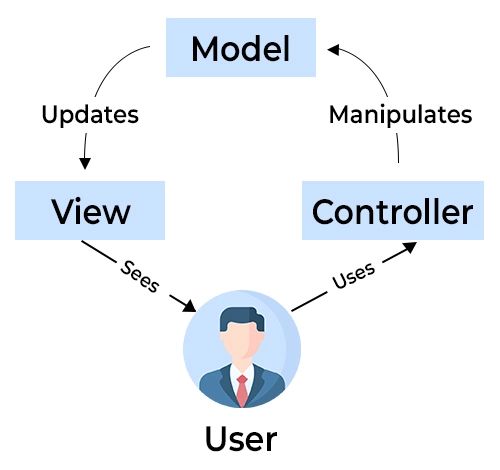
\includegraphics[width=0.4\textwidth]{slike/mvc.png} %veličina u odnosu na širinu linije
		\end{center}
		
		\begin{itemize}
			\item \textit{Model} predstavlja podatke i poslovnu logiku aplikacije. Model je odgovoran za dohvaćanje, pohranu i upravljanje podacima. Komunicira s Controllerom i obavještava ga o ažuriranim informacijama.
			
			\item \textit{View} predstavlja korisničko sučelje aplikacije. Sve što korisnik vidi je dio Viewa. On prikazuje podatke koje dobiva od Modela.
			
			\item \textit{Controller} je posrednik između Modela i Viewa. Prima korisničke zahtjeve iz Viewa, interpretira ih i odabire odgovarajuće akcije. Ovisno o korisničkom zahtjevu, Controller može ažurirati Model (kao što je spremanje podataka u bazu) i/ili ažurirati View (kao što je prikazivanje novih podataka na web stranici). Controller šalje informacije od Viewa prema Modelu, a zatim ažurirane podatke iz Modela šalje natrag Viewu za prikaz korisnicima.
		\end{itemize}
		
		 
		Aplikacija ima slojeve frontend i backend, te bazu podataka. Baza podataka zadužena za pohranu podataka naše web aplikacije je PostgreSQL s kojom smo se upoznali na predmetu Baze podataka. To je moćna relacijska baza podataka koja podržava kompleksne SQL upite i omogućuje efikasno pohranjivanje podataka u tablicama. Osim toga, osigurava konzistentnost i pouzdanost podataka. Iz nje backend sloj dohvaća podatke koristeći radni okvir Spring Boot. Ona olakšava brzi razvoj backenda jer Spring Data JPA omogućuje jednostavno rukovanje podacima putem Java objekata, čime se smanjuje količina potrebnog SQL koda. Također omogućuje lak prijenos podataka između frontend i backend slojeva. Za frontend sloj koji korisnicima prikazuje podatke koje dobiva iz backenda putem API-a koristimo Angular. U kombinaciji sa Spring Boot-om i PostgreSQL-om, Angular je moćni radni okvir koja olakšava izradu modernih, skalabilnih, i korisnički prijateljskih web aplikacija. Temelji se na komponentnoj arhitekturi, što olakšava razdvajanje funkcionalnosti i ponovnu upotrebu koda. Komponente su samostalne i mogu se lako integrirati. Najveća prednost Angulara je što koristi HTML, CSS, te Typescript, jezike koji su poznati svim članovima tima.

		

				
		\section{Baza podataka}
			
			
			
		Za potrebe našeg sustava koristit ćemo relacijsku bazu podataka koja svojom strukturom olakšava modeliranje stvarnog svijeta. Gradivna jedinka baze je relacija, odnosno tablica koja je definirana svojim imenom i skupom atributa. Zadaća baze podataka je brza i jednostavna pohrana, izmjena i dohvat podataka za daljnju obradu.
		Baza podataka ove aplikacije sastoji se od sljedećih entiteta:
		\begin{itemize}
			\item Status
			\item Client
			\item StationLead
			\item Station
			\item Request
			\item Researcher
			\item ActionComment
			\item Action
			\item ExplorerAction
			\item Explorer
			\item ExplorerLocation
			\item AnimalComment
			\item Animal
			\item AnimalLocation
			\item Vehicle
			\item EducatedFor
			\item Task
			\item Token
		\end{itemize}
		
			\subsection{Opis tablica}
				
				\textbf{Status} Ovaj entitet sadržava opis statusa korisnika. Sadrži atribute: statusId i description. Ovaj entitet u vezi je \textit{One-to-Many} s entitetom Researcher preko atributa statusId, u vezi \textit{One-to-Many} s entitetom StationLead preko atributa statusId.
				\begin{longtblr}[
					label=none,
					entry=none
					]{
						width = \textwidth,
						colspec={|X[6,l]|X[6, l]|X[20, l]|}, 
						rowhead = 1,
					} %definicija širine tablice, širine stupaca, poravnanje i broja redaka naslova tablice
					\hline \SetCell[c=3]{c}{\textbf{Status}}	 \\ \hline[3pt]
					\SetCell{LightGreen}StatusId & INT	&  	Jedinstveni identifikator statusa korisnika	\\ \hline
					Description	& VARCHAR &   Opis značenja određenog identifikatora	\\ \hline
				\end{longtblr}
				
				\textbf{Client} Ovaj entitet sadržava korisne informacije o korisniku. Sadrži atribute: clientname, password, photoURL, firstName, lastName, email. Ovaj entitet u vezi je \textit{One-to-One} s entitetom Researcher preko atributa clientname, u vezi \textit{One-to-Many} s entitetom ActionComment preko atributa clientname, u vezi \textit{One-to-One} s entitetom StationLead preko atributa clientname, u vezi \textit{One-to-One} s entitetom Explorer preko atributa clientname.
				\begin{longtblr}[
					label=none,
					entry=none
					]{
						width = \textwidth,
						colspec={|X[6,l]|X[6, l]|X[20, l]|}, 
						rowhead = 1,
					} %definicija širine tablice, širine stupaca, poravnanje i broja redaka naslova tablice
					\hline \SetCell[c=3]{c}{\textbf{Client}}	 \\ \hline[3pt]
					\SetCell{LightGreen}Client & VARCHAR	&  Jedinstveno korisničko ime korisnika  	\\ \hline
					Password	& VARCHAR &   Šifra profila korisnika	\\ \hline 
					PhotoURL & VARCHAR &  URL link slike korisnika \\ \hline 
					FirstName & VARCHAR	&  	Ime korisnika	\\ \hline 
					LastName & VARCHAR	&  	Prezime korisnika	\\ \hline
					Email & VARCHAR	&  	Jedinstveni Email korisnika	\\ \hline
				\end{longtblr}
				
				\textbf{StationLead} Ovaj entitet je razdvojeni entitet entiteta Client koji sadrži atribut poseban za voditelja koji govori koju stanicu vodi (stationId), također sadrži i atribute clientname i statusId. Ovaj entitet u vezi je \textit{One-to-One} s entitetom Client preko atributa clientname, u vezi \textit{One-to-One} s entitetom Station preko atributa stationId, u vezi \textit{Many-to-One} s entitetom Status preko atributa statusId, u vezi \textit{One-to-Many} s entitetom Request preko atributa clientname.
				\begin{longtblr}[
					label=none,
					entry=none
					]{
						width = \textwidth,
						colspec={|X[6,l]|X[6, l]|X[20, l]|}, 
						rowhead = 1,
					} %definicija širine tablice, širine stupaca, poravnanje i broja redaka naslova tablice
					\hline \SetCell[c=3]{c}{\textbf{StationLead}}	 \\ \hline[3pt]
					\SetCell{LightBlue} Clientname	& VARCHAR &   korisničko ime voditelja, (client.clientname)	\\ \hline 
					\SetCell{LightBlue} StationId	& INT &   Identifikator postaje koju voditelj vodi, (station.stationId)\\ \hline 
					\SetCell{LightBlue} StatusId	& INT &   Identifikator statusa profila korisnika (verified, declined, pending), (status.statusId)	\\ \hline 
				\end{longtblr}
				
				\textbf{Station} Ovaj entitet sadržava sve važne informacije o postaji. Sadrži atribute: stationId, radius, stationName, stationStatus, Location. U vezi je \textit{One-to-One} s entitetom StationLead preko atributa stationId, u vezi \textit{One-to-Many} s entitetom Explorer preko atributa stationId.
				\begin{longtblr}[
					label=none,
					entry=none
					]{
						width = \textwidth,
						colspec={|X[6,l]|X[6, l]|X[20, l]|}, 
						rowhead = 1,
					} %definicija širine tablice, širine stupaca, poravnanje i broja redaka naslova tablice
					\hline \SetCell[c=3]{c}{\textbf{Station}}	 \\ \hline[3pt]
					\SetCell{LightGreen}StationId & INT	&  	Jedinstveni identifikator stanice\\ \hline
					Radius	& INT &   Polumjer kruga koji označava stanicu izražen u metrima	\\ \hline 
					StationName & VARCHAR &  Naziv stanice \\ \hline 
					StationStatus & VARCHAR	&  	Status stanice, može biti zauzeta (ima voditelja) ili slobodna (nema voditelja)	\\ \hline 
					Center	& VARCHAR &   Lokacija središta stanice	\\ \hline	 
				\end{longtblr}
				
				\textbf{Request} Ovaj entitet sadržava informacije o zahtjevu koji istraživač šalje voditelju postaje. Sadrži atribute: requestId, status zahtjeva, numOfPeople, researcher i stationLead. U vezi je \textit{Many-to-One} s entitetom Researcher preko atributa researcher, u vezi \textit{Many-to-One} s entitetom StationLead preko atributa stationLead.
				\begin{longtblr}[
					label=none,
					entry=none
					]{
						width = \textwidth,
						colspec={|X[6,l]|X[6, l]|X[20, l]|}, 
						rowhead = 1,
					} %definicija širine tablice, širine stupaca, poravnanje i broja redaka naslova tablice
					\hline \SetCell[c=3]{c}{\textbf{Request}}	 \\ \hline[3pt]
					\SetCell{LightGreen} RequestId	& INT &   Jedinstveni identifikator zahtjeva	\\ \hline
					Status	& VARCHAR &   Status zahtjeva, može biti odobren, odbijen ili u obradi.	\\ \hline
					NumOfPeople & INT &   Broj ljudi koji istraživač zahtjeva od voditelja	\\ \hline
					\SetCell{LightBlue} Researcher	& VARCHAR &   Identifikator istraživača koji šalje zahtjev, (researcher.clientname)	\\ \hline
					\SetCell{LightBlue} StationLead	& VARCHAR &   Identifikator voditelja koji prima zahtjev, (stationLead.clientname)	\\ \hline 
				\end{longtblr}
				
				\textbf{Researcher} Ovaj entitet je razdvojeni entitet entiteta Client koji sadrži atribute: clientname istraživača i statusId. U vezi je \textit{One-to-One} s entitetom Client preko atributa clientname, u vezi \textit{Many-to-One} s entitetom Status preko atributa statusId, u vezi \textit{One-to-Many} s entitetom Request preko atributa clientname, u vezi \textit{One-to-Many} s entitetom Action preko atributa clientname.
				\begin{longtblr}[
					label=none,
					entry=none
					]{
						width = \textwidth,
						colspec={|X[6,l]|X[6, l]|X[20, l]|}, 
						rowhead = 1,
					} %definicija širine tablice, širine stupaca, poravnanje i broja redaka naslova tablice
					\hline \SetCell[c=3]{c}{\textbf{Researcher}}	 \\ \hline[3pt]
					\SetCell{LightBlue}Clientname & VARCHAR	&  korisničko ime istraživača, (client.clientname)\\ \hline
					\SetCell{LightBlue} StatusId	& INT &   Identifikator statusa istraživača (verified, declined, pending), (status.statusId)	\\ \hline 
				\end{longtblr}
				
				\textbf{ActionComment} Ovaj entitet sadrži informacije o komentarima ostavljenima na određenoj akciji. Sadrži atribute: CommentId, description, CommentTS, username i actionId akcije kojoj pripada. U vezi je \textit{Many-to-One} s entitetom Client preko atributa clientname, u vezi \textit{Many-to-One} s entitetom Action preko atributa actionId.
				\begin{longtblr}[
					label=none,
					entry=none
					]{
						width = \textwidth,
						colspec={|X[6,l]|X[6, l]|X[20, l]|}, 
						rowhead = 1,
					} %definicija širine tablice, širine stupaca, poravnanje i broja redaka naslova tablice
					\hline \SetCell[c=3]{c}{\textbf{ActionComment}}	 \\ \hline[3pt]
					\SetCell{LightGreen}CommentId & INT	&  	Jedinstveni identifikator komentara	\\ \hline
					Description	& VARCHAR & Sadržaj komentara	\\ \hline 
					CommentTS & TIMESTAMP &  Vrijeme postavljanja komentara \\ \hline
					Location & VARCHAR &  Lokacija postavljanja komentara \\ \hline 
					\SetCell{LightBlue} Clientname	& VARCHAR &  Identifikator korisnika koji je postavio komentar, (client.clientname)	\\ \hline
					\SetCell{LightBlue} ActionId	& INT &   Identifikator akcije na koju je postavljen komentar, (action.actionId)	\\ \hline 
				\end{longtblr}
				
				\textbf{Action} Ovaj entitet opisuje koji istraživač je pokrenuo određenu akciju. Ima atribute: actionId, researcher, title i description. U vezi je \textit{Many-to-One} s entitetom Researcher preko atributa researcher. U vezi \textit{One-to-Many} s entitetom ActionComment preko atributa actionId, u vezi \textit{One-to-Many} s entitetom ExplorerAction preko atributa actionId, u vezi \textit{One-to-Many} s entitetom Task preko atributa actionId.
				\begin{longtblr}[
					label=none,
					entry=none
					]{
						width = \textwidth,
						colspec={|X[6,l]|X[6, l]|X[20, l]|}, 
						rowhead = 1,
					} %definicija širine tablice, širine stupaca, poravnanje i broja redaka naslova tablice
					\hline \SetCell[c=3]{c}{\textbf{Action}}	 \\ \hline[3pt]
					\SetCell{LightGreen} ActionId & INT	&  	Jedinstveni identifikator akcije  	\\ \hline
					\SetCell{LightBlue} Researcher	& VARCHAR &   Identifikator istraživača koji je započeo akciju, (researcher.clientname)	\\ \hline 
					\SetCell{LightBlue} Title & VARCHAR	&  	Naslov akcije  	\\ \hline
					\SetCell{LightBlue} Description	& VARCHAR &   Opis započete akcije	\\ \hline
				\end{longtblr}
				
				\textbf{ExplorerAction} Ovaj entitet opisuje tragača i akciju na kojoj se nalazio. Ima atribute: explorer i actionId. U vezi je \textit{Many-to-One} s entitetom Explorer preko atributa clientname, u vezi \textit{Many-to-One} s entitetom Action preko atributa actionId.
				\begin{longtblr}[
					label=none,
					entry=none
					]{
						width = \textwidth,
						colspec={|X[6,l]|X[6, l]|X[20, l]|}, 
						rowhead = 1,
					} %definicija širine tablice, širine stupaca, poravnanje i broja redaka naslova tablice
					\hline \SetCell[c=3]{c}{\textbf{ExplorerAction}}	 \\ \hline[3pt]
					\SetCell{LightBlue} Explorer	& VARCHAR &   Korisničko ime tragača, (explorer.clientname)	\\ \hline 
					\SetCell{LightBlue} ActionId	& INT &   Identifikator akcije tragača, (action.actionId)	\\ \hline
				\end{longtblr}
				
				\textbf{Explorer} Ovaj entitet je razdvojeni entitet entiteta Client koji sadrži atribute: clientname i stationId. U vezi je \textit{One-to-One} s entitetom Client preko atributa clientname, u vezi \textit{One-to-Many} s entitetom ExplorerAction preko atributa clientname, u vezi \textit{One-to-Many} s entitetom EducatedFor preko atributa clientname, u vezi \textit{One-to-Many} s entitetom Task preko atributa clientname, u vezi \textit{One-to-Many} s entitetom AnimalComment preko atributa clientname, u vezi \textit{One-to-Many} s entitetom ExplorerLocation preko atributa clientname, u vezi \textit{Many-to-One} s entitetom Station preko atributa stationId.
				\begin{longtblr}[
					label=none,
					entry=none
					]{
						width = \textwidth,
						colspec={|X[6,l]|X[6, l]|X[20, l]|}, 
						rowhead = 1,
					} %definicija širine tablice, širine stupaca, poravnanje i broja redaka naslova tablice
					\hline \SetCell[c=3]{c}{\textbf{Explorer}}	 \\ \hline[3pt]
					\SetCell{LightBlue}Clientname & VARCHAR	&  Korisničko ime tragača, (client.clientname)	\\ \hline
					\SetCell{LightBlue} StationId	& INT &   Identifikator postaje kojoj pripada, (station.stationId)	\\ \hline 
				\end{longtblr}
				
				\textbf{ExplorerLocation} Ovaj entitet sadrži lokaciju tragača u određenom vremenu. Ima atribute: LocationTS, explorer i Location. U vezi je \textit{Many-to-One} s entitetom Explorer preko atributa client.name.
				\begin{longtblr}[
					label=none,
					entry=none
					]{
						width = \textwidth,
						colspec={|X[6,l]|X[6, l]|X[20, l]|}, 
						rowhead = 1,
					} %definicija širine tablice, širine stupaca, poravnanje i broja redaka naslova tablice
					\hline \SetCell[c=3]{c}{\textbf{ExplorerLocation}}	 \\ \hline[3pt]
					\SetCell{LightGreen} Location	& VARCHAR &   Lokacija tragača	\\ \hline
					LocationTS & TIMESTAMP	&  Vrijeme očitanja lokacije tragača\\ \hline
					\SetCell{LightBlue} Explorer	& VARCHAR &   Korisničko ime tragača, (explorer.clientname)	\\ \hline 
					 
				\end{longtblr}
				
				\textbf{AnimalComment} Ovaj entitet sadrži sve komentare o očitanim životinjama. Ima atribute: commentId, commentTS, comment, explorer, animalId. U vezi je \textit{Many-to-One} s entitetom Explorer preko atributa explorer, u vezi \textit{Many-to-One} s entitetom Animal preko atributa animalId.
				\begin{longtblr}[
					label=none,
					entry=none
					]{
						width = \textwidth,
						colspec={|X[6,l]|X[6, l]|X[20, l]|}, 
						rowhead = 1,
					} %definicija širine tablice, širine stupaca, poravnanje i broja redaka naslova tablice
					\hline \SetCell[c=3]{c}{\textbf{AnimalComment}}	 \\ \hline[3pt]
					\SetCell{LightGreen}CommentId & INT	&  Jedinstveni identifikator komentara	\\ \hline
					CommentTS	& TIMESTAMP &   Vrijeme objave komentara	\\ \hline 
					Comment & VARCHAR & Sadržaj komentara  \\ \hline 
					\SetCell{LightBlue} Explorer	& VARCHAR &   Korisničko ime tragača koji je komentirao, (explorer.clientname)	\\ \hline 
					\SetCell{LightBlue} AnimalId	& INT &   Identifikator komentirane životinje, (animal.animalId)	\\ \hline 
				\end{longtblr}
				
				\textbf{Animal} Ovaj entitet sadrži sve bitne informacije o očitanoj životinji. Ima atribute: animalId, species, description, photoURL. U vezi je \textit{One-to-Many} s entitetom AnimalComment preko atributa animalId, u vezi \textit{One-to-Many} s entitetom AnimalLocation preko atributa animalId.
				\begin{longtblr}[
					label=none,
					entry=none
					]{
						width = \textwidth,
						colspec={|X[6,l]|X[6, l]|X[20, l]|}, 
						rowhead = 1,
					} %definicija širine tablice, širine stupaca, poravnanje i broja redaka naslova tablice
					\hline \SetCell[c=3]{c}{\textbf{Animal}}	 \\ \hline[3pt]
					\SetCell{LightGreen}AnimalId & INT	&  	Jedinstveni identifikator očitane životinje  	\\ \hline
					Species	& VARCHAR &   Vrsta životinje	\\ \hline 
					Description & VARCHAR & Opis životinje  \\ \hline 
					PhotoURL & VARCHAR	&  	URL slike životinje	\\ \hline
				\end{longtblr}
				
				\textbf{AnimalLocation} Ovaj entitet sadrži lokaciju životinje u određenom vremenu. Ima atribute: LocationTS, Location, AnimalId. U vezi je \textit{Many-to-One} s entitetom Animal preko atributa animalId.
				\begin{longtblr}[
					label=none,
					entry=none
					]{
						width = \textwidth,
						colspec={|X[6,l]|X[6, l]|X[20, l]|}, 
						rowhead = 1,
					} %definicija širine tablice, širine stupaca, poravnanje i broja redaka naslova tablice
					\hline \SetCell[c=3]{c}{\textbf{AnimalLocation}}	 \\ \hline[3pt]
					\SetCell{LightGreen} Location	& VARCHAR &   Lokacija životinje	\\ \hline
					LocationTS & TIMESTAMP	&  Vrijeme zapisa lokacije životinje	\\ \hline
					\SetCell{LightBlue} AnimalId	& INT &   Identifikator očitane životinje, (animal.animalId)	\\ \hline 
				\end{longtblr}
				
				\textbf{EducatedFor} Ovaj entitet opisuje koji tragači znaju upravljati kojim vozilima. Ima atribute: vehicleId i explorer. U vezi je \textit{Many-to-One} s entitetom Explorer preko atributa clientname, u vezi \textit{Many-to-One} s entitetom Vehicle preko atributa vehicleId.
				\begin{longtblr}[
					label=none,
					entry=none
					]{
						width = \textwidth,
						colspec={|X[6,l]|X[6, l]|X[20, l]|}, 
						rowhead = 1,
					} %definicija širine tablice, širine stupaca, poravnanje i broja redaka naslova tablice
					\hline \SetCell[c=3]{c}{\textbf{EducatedFor}}	 \\ \hline[3pt] 
					\SetCell{LightBlue} VehicleId	& INT &   Identifikator vozila kojeg tragač zna voziti, (vehicle.vehicleId)	\\ \hline 
					\SetCell{LightBlue} Explorer	& VARCHAR &   Korisničko ime tragača, (explorer.clientname)	\\ \hline 
				\end{longtblr}
				
				\textbf{Vehicle} Ovaj entitet sadrži nazive vozila. Ima atribute: vehicleId, vehicleType. U vezi je \textit{One-to-Many} s entitetom Task preko atributa vehicleId, u vezi \textit{One-to-Many} s entitetom EducatedFor preko atributa vehicleId.
				\begin{longtblr}[
					label=none,
					entry=none
					]{
						width = \textwidth,
						colspec={|X[6,l]|X[6, l]|X[20, l]|}, 
						rowhead = 1,
					} %definicija širine tablice, širine stupaca, poravnanje i broja redaka naslova tablice
					\hline \SetCell[c=3]{c}{\textbf{Vehicle}}	 \\ \hline[3pt]
					\SetCell{LightGreen}VehicleId & INT	&  Jedinstveni identifikator vozila	\\ \hline
					VehicleType	& VARCHAR &   Naziv vozila	\\ \hline 
				\end{longtblr}
				
				\textbf{Task} Ovaj entitet sadrži sve bitne informacije o zadatku. Ima atribute: taskId, description, startLocation, endLocation, taskTS, actionId, explorer, vehicleId. U vezi je \textit{Many-to-One} s entitetom Action preko atributa actionId, u vezi \textit{Many-to-One} s entitetom Explorer preko atributa clientname, u vezi \textit{Many-to-One} s entitetom Vehicle preko atributa vehicleId.
				\begin{longtblr}[
					label=none,
					entry=none
					]{
						width = \textwidth,
						colspec={|X[6,l]|X[6, l]|X[20, l]|}, 
						rowhead = 1,
					} %definicija širine tablice, širine stupaca, poravnanje i broja redaka naslova tablice
					\hline \SetCell[c=3]{c}{\textbf{Task}}	 \\ \hline[3pt]
					\SetCell{LightGreen}TaskId & INT	&  	Jedinstveni identifikator zadatka\\ \hline
					Description	& VARCHAR &   Opis zadatka	\\ \hline 
					StartLocation & VARCHAR &  Lokacija početka zadatka \\ \hline 
					EndLocation & VARCHAR	&  	Lokacija završetka zadatka	\\ \hline 
					TaskTS & TIMESTAMP	&  	Vrijeme početka zadatka	\\ \hline 
					\SetCell{LightBlue} ActionId	& INT &   Identifikator akcije kojoj pripada zadatak, (action.actionId)	\\ \hline
					\SetCell{LightBlue} Explorer	& VARCHAR &   Korisničko ime tragača koji izvršava zadatak	\\ \hline 
					\SetCell{LightBlue} VehicleId	& INT &   Identifikator vozila s kojim se obavlja zadatak, (vehicle.vehicleId)	\\ \hline
				\end{longtblr}
				
				\textbf{Token} Ovaj entitet sve podatke o tokenu koji se generira pri registraciji ili prijavi korisnika u sustav. Ima atribute: tokenId, tokenType, revoked, expired, clientname. U vezi je \textit{Many-to-One} s entitetom Client preko atributa clientname.
			     \begin{longtblr}[
					label=none,
					entry=none
					]{
						width = \textwidth,
						colspec={|X[6,l]|X[6, l]|X[20, l]|}, 
						rowhead = 1,
					} %definicija širine tablice, širine stupaca, poravnanje i broja redaka naslova tablice
					\hline \SetCell[c=3]{c}{\textbf{Token}}	 \\ \hline[3pt]
					\SetCell{LightGreen}TokenkId & INT	&  	Jedinstveni identifikator tokena\\ \hline
					TokenType & VARCHAR & Tip generiranog tokena \\ \hline
					Token & VARCHAR & Generirani token \\ \hline
					Revoked & BOOLEAN & Zastavica koja daje informaciju o tome je li token opozvan \\ \hline
					Expired & BOOLEAN & Zastavica koja daje informaciju o tome je li token istekao \\ \hline
					\SetCell{LightBlue} Client	& VARCHAR &   Korisničko ime klijenta koji koristi token, (client.clientname)	\\ \hline
					
				\end{longtblr}
				
				
			
			\subsection{Dijagram baze podataka}
				\begin{figure}[H]
					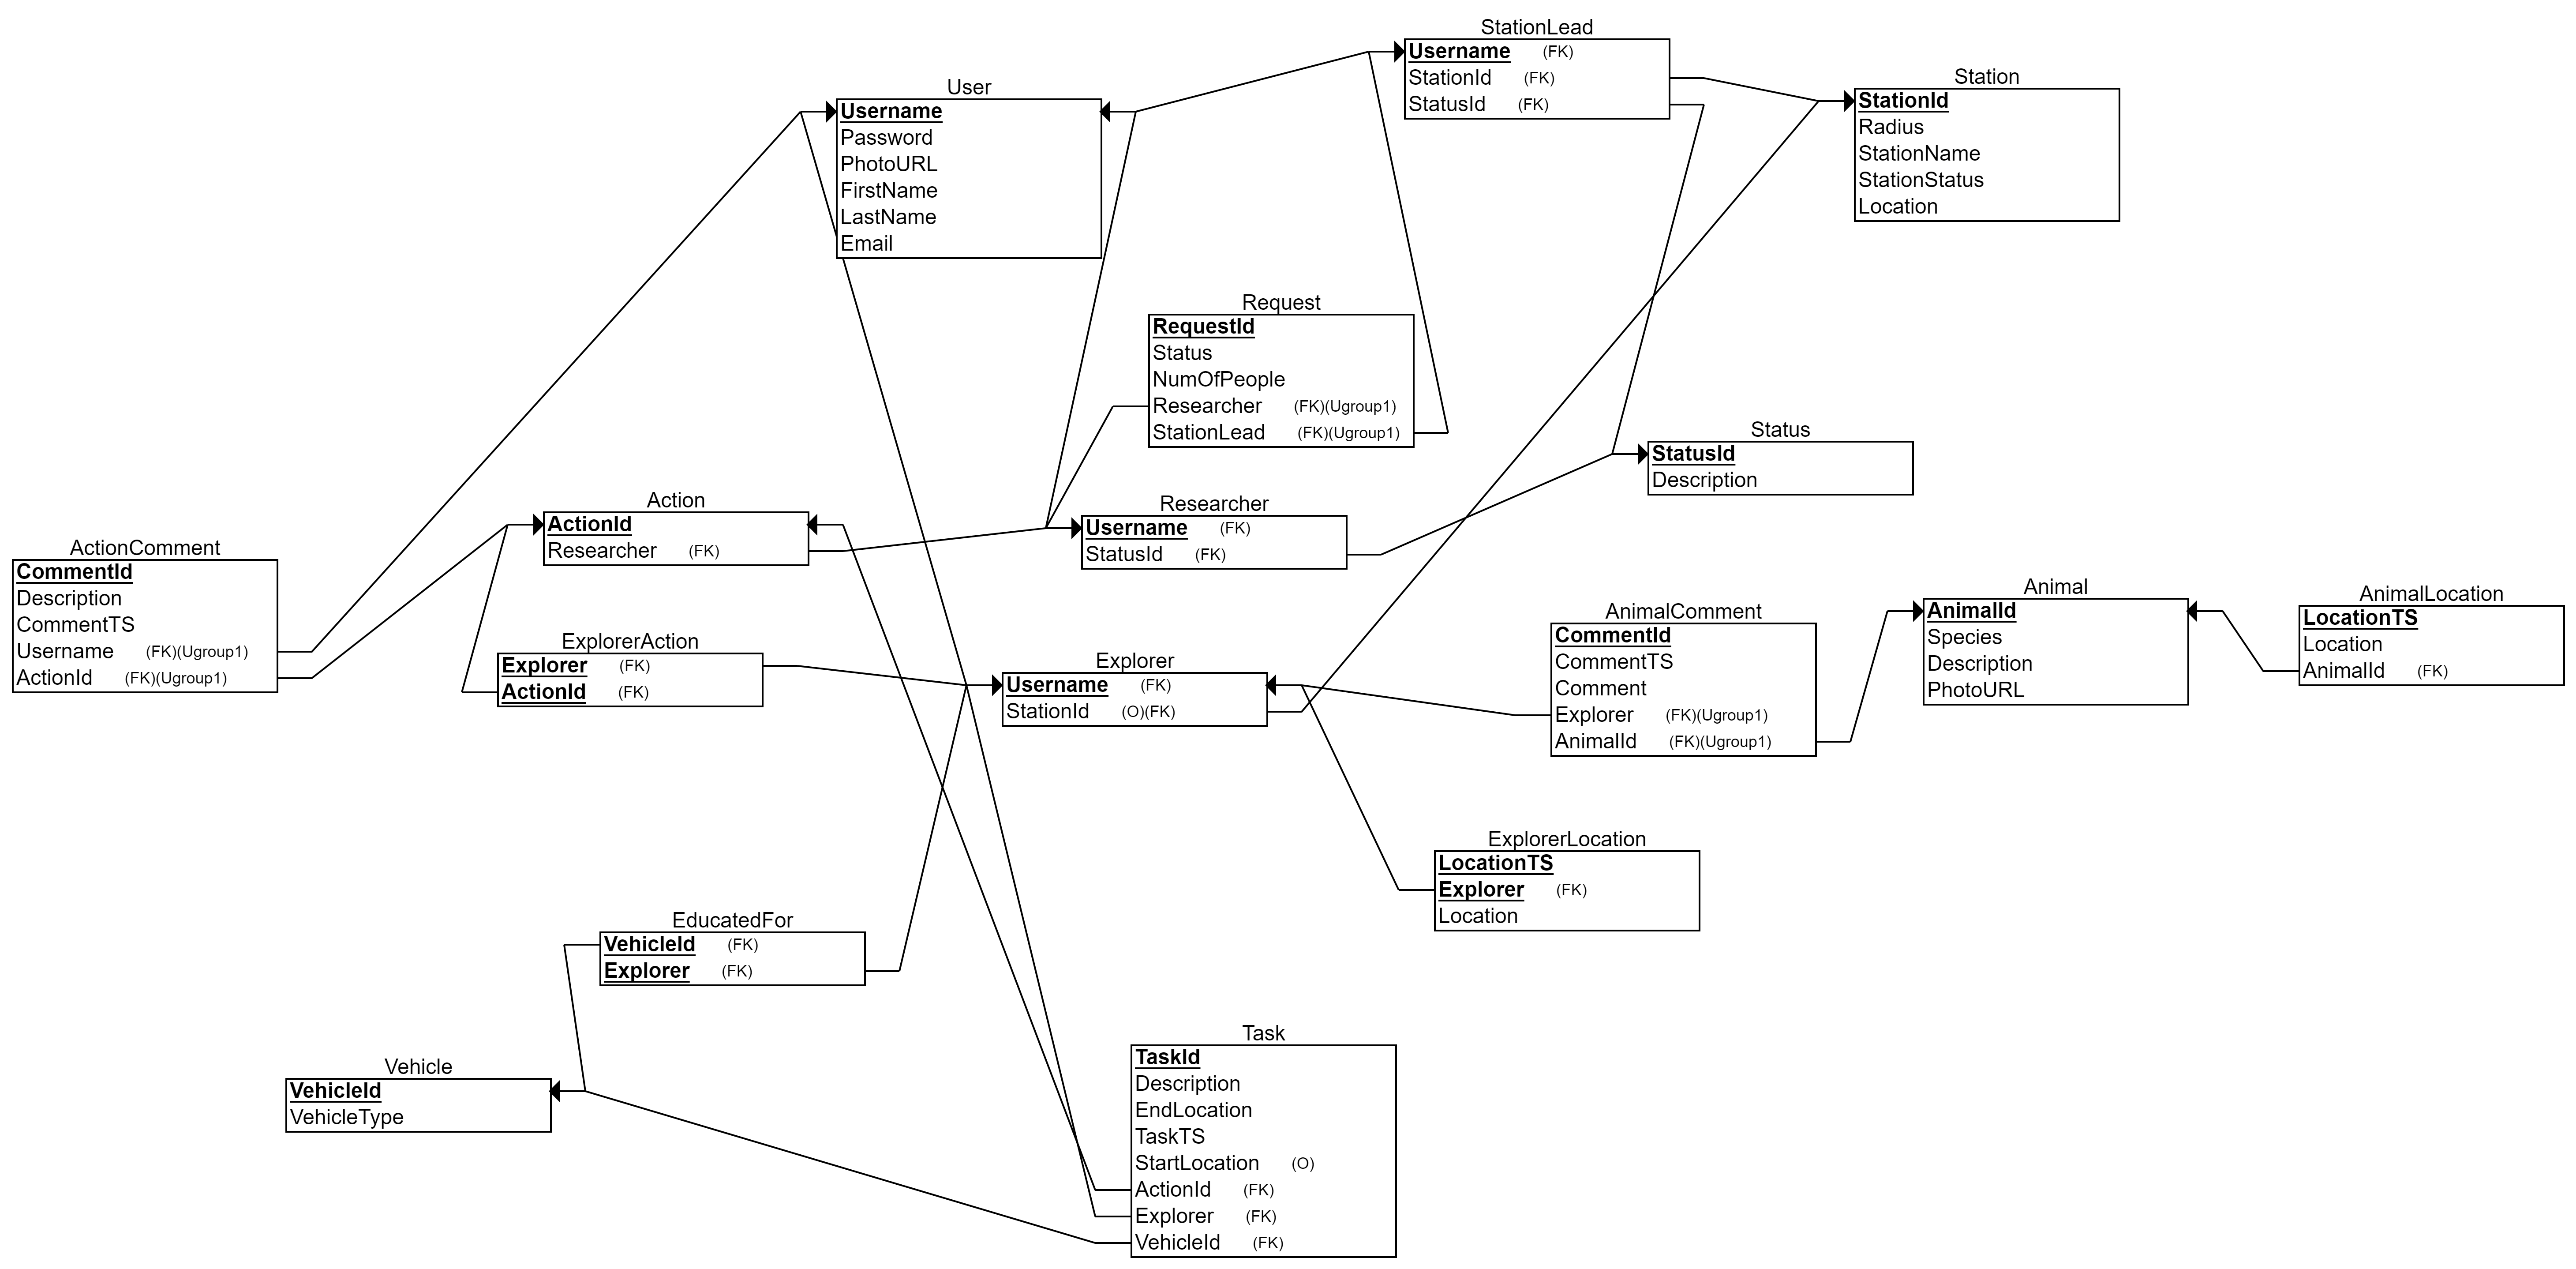
\includegraphics[width=\textwidth]{slike/dijagram_baze.PNG} %veličina u odnosu na širinu linije
					\caption{Dijagram baze podataka}
					\label{fig:dijagram_baze} %label mora biti drugaciji za svaku sliku
				\end{figure}
			
			\eject
			
			
		\section{Dijagram razreda}
		
			Na slikama 4.2, 4.3 predstavljeni su razredi koji se odnose na backend komponentu MVC obrasca. Razredi na slici 4.2 nasljeđuju Controller razred. U tim razredima, metode rukuju s Data Transfer Object (DTO), a podaci se dohvaćaju kroz metode definirane u Model razredima. Funkcije implementirane u Controller razredima generiraju JSON datoteke s HTML status kodovima.S ciljem olakšane organizacije, razredi su strukturirani prema ovlastima određenih korisnika, a unutar dijagrama su predstavljene isključivo povezanosti između razreda unutar istog dijela dijagrama. Iz naziva i tipova atributa u razredima može se zaključiti vrsta povezanosti između različitih razreda.
			
			\vspace{90pt}
			
			
			\begin{figure}[H]
				\centering
				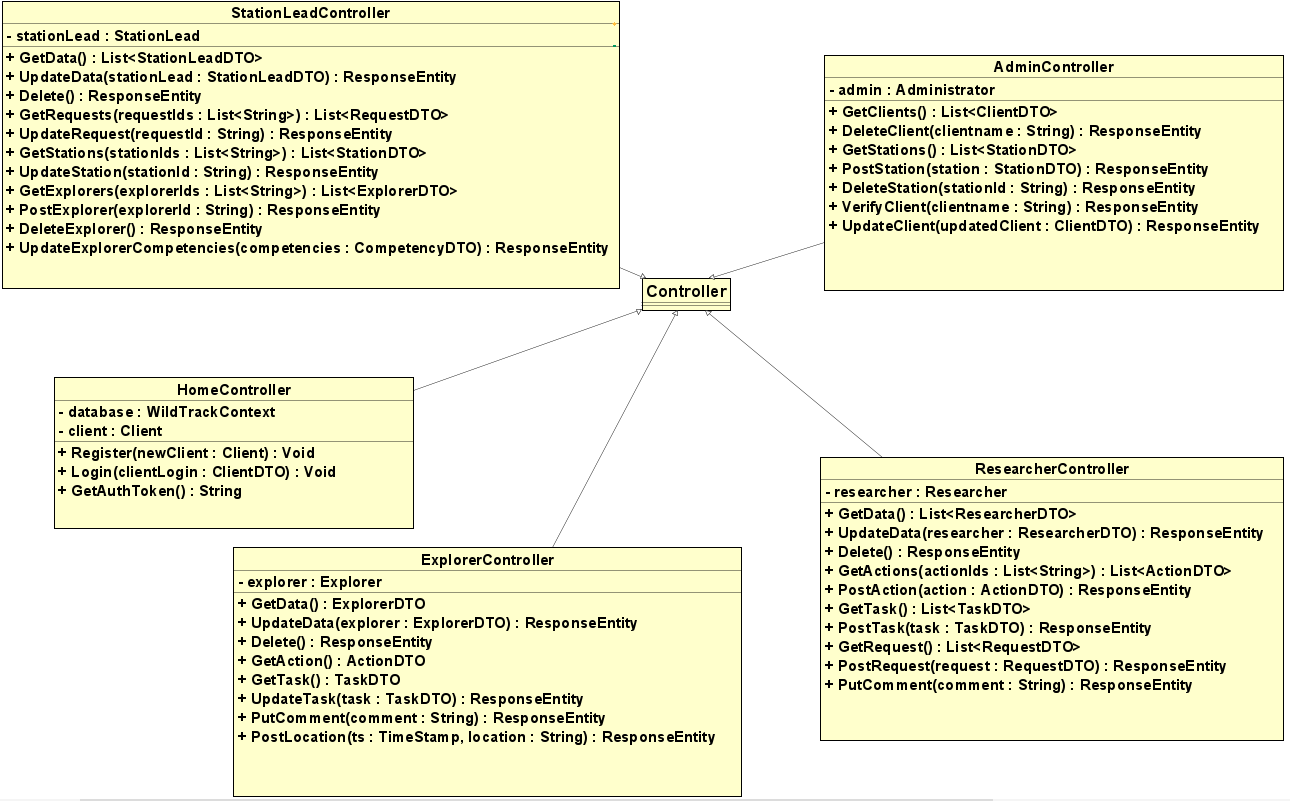
\includegraphics[width=\textwidth]{slike/Controlleri.PNG}
				\caption{Dijagram razreda - dio Controllers}
				\label{fig:dijagram_baze}
			\end{figure}
			
			
			\begin{figure}[H]
				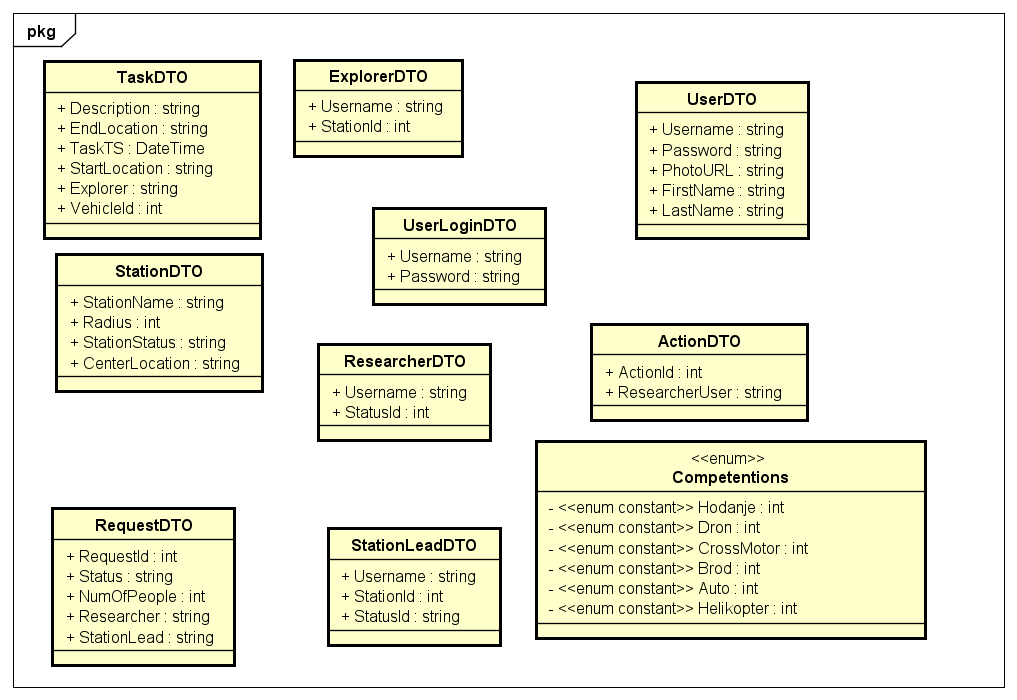
\includegraphics[width=\textwidth]{slike/Class_Diagram0.PNG} %veličina u odnosu na širinu linije
				\caption{Dijagram razreda - dio Data transfer objects}
				\label{fig:dijagram_baze} %label mora biti drugaciji za svaku sliku
			\end{figure}
			
			\vspace{36pt}
			
			Implementirane metode direktno komuniciraju s bazom podataka te vraćaju tražene podatke. Razred User predstavlja neregistriranog korisnika koji se može registrirati u sustav unoseći osnovne informacije. Razred UserLogin predstavlja već registriranog korisnika koji se može prijaviti u sustav unoseći korisničko ime i lozinku. Razred Reasearcher predstavlja istraživača koji ima ovlasti kreiranja novih akcija i slanja zahtjeva za tragačima voditelju postaje. Razred StationLead predstavlja voditelja postaje koji ima ovlasti odabrati postaju i tragače svoje vlastite postaje. Razred Explorer predstavlja tragača koji obavlja zadatke koje mu je dodijelio istraživač. Razred Administrator predstavlja administratora sustava koji ima najveće ovlasti.
			
			\vspace{36pt}
		
		\section{Dijagram stanja}
			
			Dijagram stanja jasno prikazuje kako sustav ili njegovi dijelovi prelaze iz jednog stanja u drugo kao odgovor na vanjske ili unutarnje događaje. Na slici 4.4 prikazan je dijagram stanja za registriranog korisnika. Klikom na "Moj Profil" prikazuju mu se njegovi podaci, koje može urediti ili brisati. Ovisno o ulozi koju je odabrao pri registraciji, korisnik može biti voditelj, tragač ili istraživač. Kao voditelj, može odabrati jednu od ponuđenih slobodnih postaja. Nakon toga, ima mogućnost odabrati tragače svoje postaje, te istovremeno voditelj definira na koji način su njegovi tragači osposobljeni za izvođenje istraživanja. Voditelj također ima opciju prihvatiti ili odbiti zahtjev koji mu je poslao istraživač. Istraživač kreira akciju i zatim šalje zahtjev voditelju. Nakon što mu se odobri zahtjev, on podijeli zadatke tragačima zaduženima za tu akciju. Istraživaču se na ekranu prikazuje karta s informacijama o pozicijama životinja i tragača. Također, ima mogućnost ostavljati komentare tragačima na akciji. Tragač na karti može vidjeti svoje zadatke (usput ih obavljati), životinje te ostale tragače na istoj akciji. Prilikom obavljanja zadatka može ostaviti komentare ostalim tragačima.
			
			\begin{figure}[H]
				\centering
				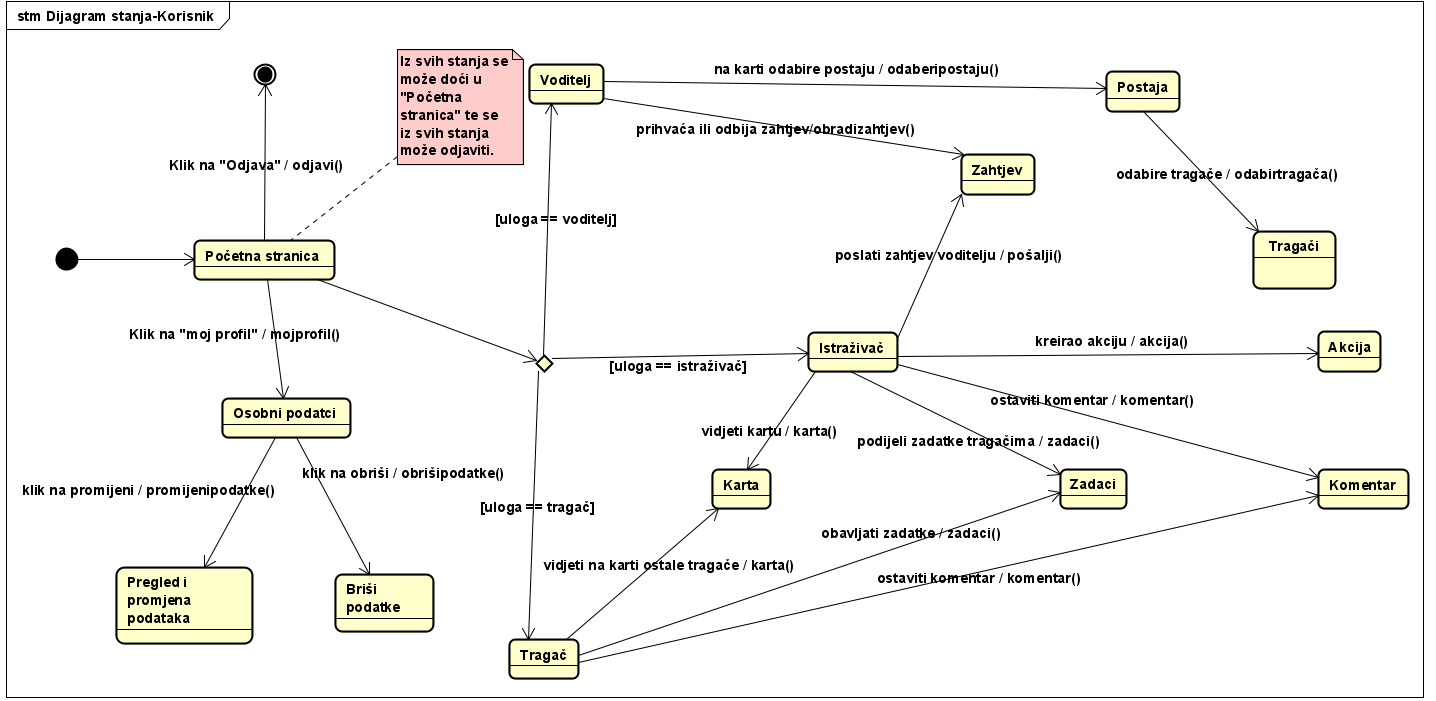
\includegraphics[width=\textwidth]{slike/Dijagram_stanja.PNG}
				\caption{Dijagram stanja }
				\label{fig:dijagram_baze}
			\end{figure}
			
			\eject 
		
		\section{Dijagram aktivnosti}
			
		Dijagram aktivnosti upotrebljava se za prikaz tijeka aktivnosti, akcija i odluka procesa u sustavu. Posebno su korisni za vizualizaciju složenih ponašanja kao npr. slijedne i paralelne aktivnosti, kao i točke odlučivanja i uvjetno grananje. U modeliranju toka upravljanja svaki novi korak poduzima se nakon završenog prethodnog, a naglasak je na jednostavnosti. Na slici 4.5 prikazan je proces kreiranja akcije. Voditelj odabire postaju i tragače te im odabire kompetencije, a zatim istraživač može poslati zahtjev voditelju. U slučaju prihvaćanja zahtjeva istraživač dalje kreira akciju i dodjeljuje zadatke tragačima. Nakon što svi tragači koji sudjeluju u toj akciji obave sve svoje zadatke akcija se smatra završenom. 
		
		\begin{figure}[H]
			\centering
			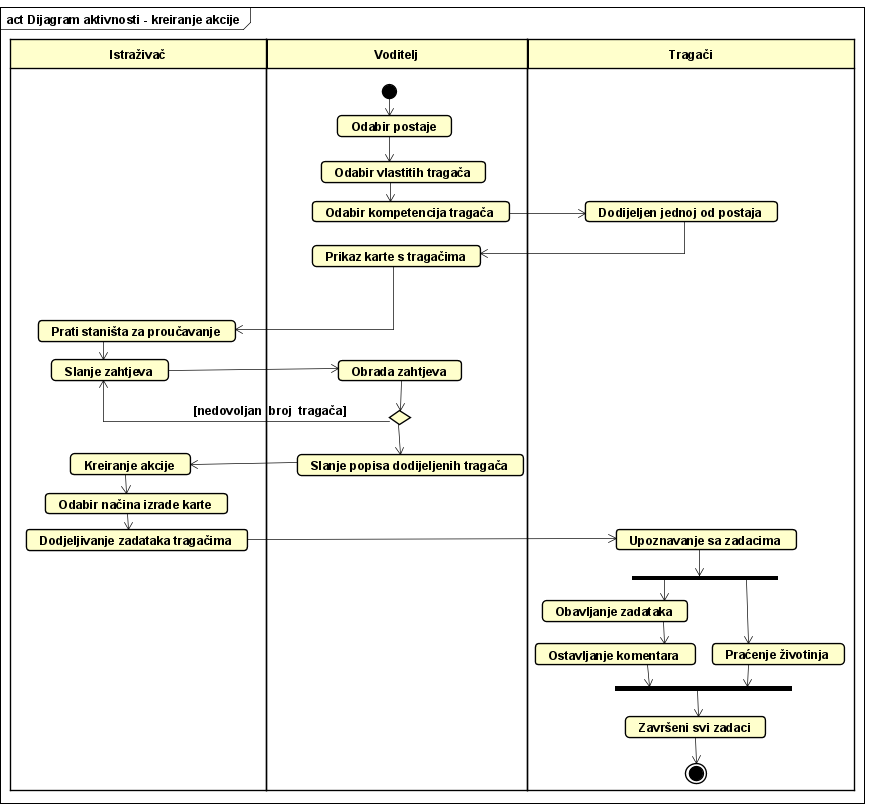
\includegraphics[width=\textwidth]{slike/Dijagram_aktivnosti.PNG}
			\caption{Dijagram aktivnosti }
			\label{fig:dijagram_baze}
		\end{figure}
			
			\eject
			
		\section{Dijagram komponenti}
		
		Na slici 4.6 prikazan je dijagram komponenti. Korisnik putem web preglednika pristupa aplikaciji putem REST API-ja. Samu aplikaciju možemo podijeliti u dvije komponente. Prva komponenta odgovara frontendu. Ona je izgrađena korištenjem Angulara. Druga komponenta odgovara backendu te je izgrađena pomoću radnog okvira Spring Boot. Komunikacija između frontenda i backenda se odvija pomoću REST API-ja. Koristimo relacijsku bazu podataka kojoj backend pristupa slanjem SQL upita.
		
		\begin{figure}[H]
			\centering
			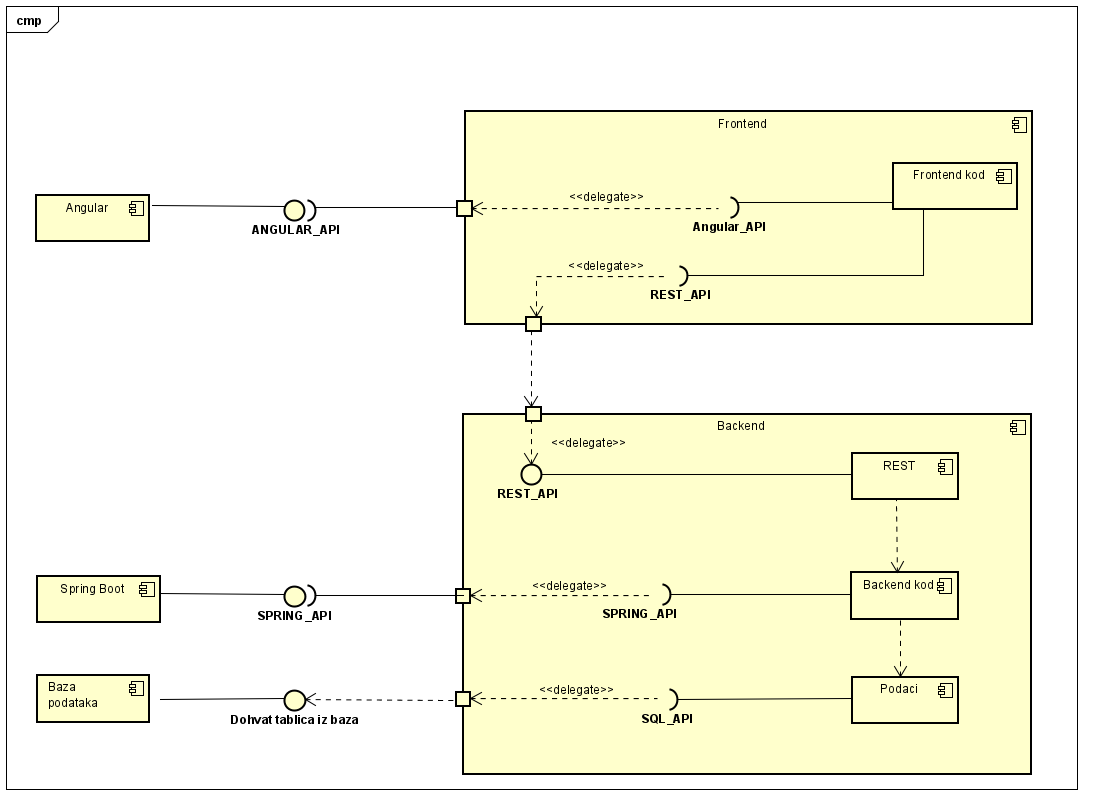
\includegraphics[width=\textwidth]{slike/Dijagram_komponenti.PNG}
			\caption{Dijagram komponenti }
			\label{fig:dijagram_baze}
		\end{figure}
	\chapter{Implementacija i korisničko sučelje}
		
		
		\section{Korištene tehnologije i alati}
		
			\textbf{\textit{dio 2. revizije}}
			
			 \textit{Detaljno navesti sve tehnologije i alate koji su primijenjeni pri izradi dokumentacije i aplikacije. Ukratko ih opisati, te navesti njihovo značenje i mjesto primjene. Za svaki navedeni alat i tehnologiju je potrebno \textbf{navesti internet poveznicu} gdje se mogu preuzeti ili više saznati o njima}.
			
			
			\eject 
		
	
		\section{Ispitivanje programskog rješenja}
			
			\textbf{\textit{dio 2. revizije}}\\
			
			 \textit{U ovom poglavlju je potrebno opisati provedbu ispitivanja implementiranih funkcionalnosti na razini komponenti i na razini cijelog sustava s prikazom odabranih ispitnih slučajeva. Studenti trebaju ispitati temeljnu funkcionalnost i rubne uvjete.}
	
			
			\subsection{Ispitivanje komponenti}
			\textit{Potrebno je provesti ispitivanje jedinica (engl. unit testing) nad razredima koji implementiraju temeljne funkcionalnosti. Razraditi \textbf{minimalno 6 ispitnih slučajeva} u kojima će se ispitati redovni slučajevi, rubni uvjeti te izazivanje pogreške (engl. exception throwing). Poželjno je stvoriti i ispitni slučaj koji koristi funkcionalnosti koje nisu implementirane. Potrebno je priložiti izvorni kôd svih ispitnih slučajeva te prikaz rezultata izvođenja ispita u razvojnom okruženju (prolaz/pad ispita). }
			
			
			
			\subsection{Ispitivanje sustava}
			
			 \textit{Potrebno je provesti i opisati ispitivanje sustava koristeći radni okvir Selenium\footnote{\url{https://www.seleniumhq.org/}}. Razraditi \textbf{minimalno 4 ispitna slučaja} u kojima će se ispitati redovni slučajevi, rubni uvjeti te poziv funkcionalnosti koja nije implementirana/izaziva pogrešku kako bi se vidjelo na koji način sustav reagira kada nešto nije u potpunosti ostvareno. Ispitni slučaj se treba sastojati od ulaza (npr. korisničko ime i lozinka), očekivanog izlaza ili rezultata, koraka ispitivanja i dobivenog izlaza ili rezultata.\\ }
			 
			 \textit{Izradu ispitnih slučajeva pomoću radnog okvira Selenium moguće je provesti pomoću jednog od sljedeća dva alata:}
			 \begin{itemize}
			 	\item \textit{dodatak za preglednik \textbf{Selenium IDE} - snimanje korisnikovih akcija radi automatskog ponavljanja ispita	}
			 	\item \textit{\textbf{Selenium WebDriver} - podrška za pisanje ispita u jezicima Java, C\#, PHP koristeći posebno programsko sučelje.}
			 \end{itemize}
		 	\textit{Detalji o korištenju alata Selenium bit će prikazani na posebnom predavanju tijekom semestra.}
			
			\eject 
		
		
		\section{Dijagram razmještaja}
			
			\textbf{\textit{dio 2. revizije}}
			
			 \textit{Potrebno je umetnuti \textbf{specifikacijski} dijagram razmještaja i opisati ga. Moguće je umjesto specifikacijskog dijagrama razmještaja umetnuti dijagram razmještaja instanci, pod uvjetom da taj dijagram bolje opisuje neki važniji dio sustava.}
			
			\eject 
		
		\section{Upute za puštanje u pogon}
		
			\textbf{\textit{dio 2. revizije}}\\
		
			 \textit{U ovom poglavlju potrebno je dati upute za puštanje u pogon (engl. deployment) ostvarene aplikacije. Na primjer, za web aplikacije, opisati postupak kojim se od izvornog kôda dolazi do potpuno postavljene baze podataka i poslužitelja koji odgovara na upite korisnika. Za mobilnu aplikaciju, postupak kojim se aplikacija izgradi, te postavi na neku od trgovina. Za stolnu (engl. desktop) aplikaciju, postupak kojim se aplikacija instalira na računalo. Ukoliko mobilne i stolne aplikacije komuniciraju s poslužiteljem i/ili bazom podataka, opisati i postupak njihovog postavljanja. Pri izradi uputa preporučuje se \textbf{naglasiti korake instalacije uporabom natuknica} te koristiti što je više moguće \textbf{slike ekrana} (engl. screenshots) kako bi upute bile jasne i jednostavne za slijediti.}
			
			
			 \textit{Dovršenu aplikaciju potrebno je pokrenuti na javno dostupnom poslužitelju. Studentima se preporuča korištenje neke od sljedećih besplatnih usluga: \href{https://aws.amazon.com/}{Amazon AWS}, \href{https://azure.microsoft.com/en-us/}{Microsoft Azure} ili \href{https://www.heroku.com/}{Heroku}. Mobilne aplikacije trebaju biti objavljene na F-Droid, Google Play ili Amazon App trgovini.}
			
			
			\eject 
	\chapter{Zaključak i budući rad}
		
		\textbf{\textit{dio 2. revizije}}\\
		
		 \textit{U ovom poglavlju potrebno je napisati osvrt na vrijeme izrade projektnog zadatka, koji su tehnički izazovi prepoznati, jesu li riješeni ili kako bi mogli biti riješeni, koja su znanja stečena pri izradi projekta, koja bi znanja bila posebno potrebna za brže i kvalitetnije ostvarenje projekta i koje bi bile perspektive za nastavak rada u projektnoj grupi.}
		
		 \textit{Potrebno je točno popisati funkcionalnosti koje nisu implementirane u ostvarenoj aplikaciji.}
		
		\eject 
	\chapter*{Popis literature}
		\addcontentsline{toc}{chapter}{Popis literature}
	 	
 		\textbf{\textit{Kontinuirano osvježavanje}}
	
		\textit{Popisati sve reference i literaturu koja je pomogla pri ostvarivanju projekta.}
		
		
		\begin{enumerate}
			
			
			\item  Programsko inženjerstvo, FER ZEMRIS, \url{http://www.fer.hr/predmet/proinz}
			
			%\item  I. Sommerville, "Software engineering", 8th ed, Addison Wesley, 2007.
			
			%\item  T.C.Lethbridge, R.Langaniere, "Object-Oriented Software Engineering", 2nd ed. McGraw-Hill, 2005.
			
			%\item  I. Marsic, Software engineering book``, Department of Electrical and Computer Engineering, Rutgers University, \url{http://www.ece.rutgers.edu/~marsic/books/SE}
			
			%\item  The Unified Modeling Language, \url{https://www.uml-diagrams.org/}
			
			%\item  Astah Community, \url{http://astah.net/editions/uml-new}
		\end{enumerate}
		
		 
	
	
	\begingroup
	\renewcommand*\listfigurename{Indeks slika i dijagrama}
	%\renewcommand*\listtablename{Indeks tablica}
	%\let\clearpage\relax
	\listoffigures
	%\vspace{10mm}
	%\listoftables
	\endgroup
	\addcontentsline{toc}{chapter}{Indeks slika i dijagrama}


	
	\eject 
		
	\chapter*{Dodatak: Prikaz aktivnosti grupe}
		\addcontentsline{toc}{chapter}{Dodatak: Prikaz aktivnosti grupe}
		
		\section*{Dnevnik sastajanja}
		
		\begin{packed_enum}
			\item  sastanak
			
			\item[] \begin{packed_item}
				\item Datum: 20. listopada 2023.
				\item Prisustvovali: E.Prpić, I.Cvijetić, S.Gašpar, I.Lisica, S.Medjaković, J.Spajić, F.Vitković
				\item Teme sastanka:
				\begin{packed_item}
					\item  sastanak s asistentom
					\item  analiza zadatka
					\item  upoznavanje s timom
					\item  odabir tehnologija i alata
					\item  prvobitna raspodjela posla po članovima (backend/frontend)
				\end{packed_item}
			\end{packed_item}
			
			\item  sastanak
			\item[] \begin{packed_item}
				\item Datum: 26. listopada 2023.
				\item Prisustvovali: E.Prpić, I.Cvijetić, S.Gašpar, I.Lisica, S.Medjaković, J.Spajić, F.Vitković
				\item Teme sastanka:
				\begin{packed_item}
					\item  brainstorming ideja
					\item  opis projektnog zadatka
					\item  definiranje funkcionalnih zahtjeva
					\item  detaljnija raspodjela posla po članovima
				\end{packed_item}
			\end{packed_item}
			
			\item  sastanak
			\item[] \begin{packed_item}
				\item Datum: 31. listopada 2023.
				\item Prisustvovali: E.Prpić, I.Cvijetić, S.Gašpar, I.Lisica, S.Medjaković, J.Spajić, F.Vitković
				\item Teme sastanka:
				\begin{packed_item}
					\item  definiranje oblikovnih obrazaca
					\item  transfer znanja
					\item  raspodjela zadataka (oblikovni obrasci, sekvencijski dijagrami, ostali zahtjevi, arhitektura i dizajn sustava)
				\end{packed_item}
			\end{packed_item}
			
			\item  sastanak
			\item[] \begin{packed_item}
				\item Datum: 1. studenog 2023.
				\item Prisustvovali: E.Prpić, I.Lisica, S.Medjaković
				\item Teme sastanka:
				\begin{packed_item}
					\item  definiranje entiteta i veza baze
					\item  izrada ER i relacijskog modela baze
				\end{packed_item}
			\end{packed_item}
			
			\item  sastanak
			\item[] \begin{packed_item}
				\item Datum: 2. studenog 2023.
				\item Prisustvovali: I.Cvijetić, F.Vitković, S.Medjaković
				\item Teme sastanka:
				\begin{packed_item}
					\item  opis oblikovnih obrazaca
					\item  proučavanje git tehnologije
				\end{packed_item}
			\end{packed_item}
			
			\item  sastanak
			\item[] \begin{packed_item}
				\item Datum: 4. studenog 2023.
				\item Prisustvovali: I.Cvijetić, F.Vitković
				\item Teme sastanka:
				\begin{packed_item}
					\item  rad na sekvencijskim dijagramima
					\item  proučavanje astah programa
				\end{packed_item}
			\end{packed_item}
			
			\item  sastanak
			\item[] \begin{packed_item}
				\item Datum: 5. studenog 2023.
				\item Prisustvovali: J.Spajić, F.Vitković
				\item Teme sastanka:
				\begin{packed_item}
					\item  dijagrami obrazaca uporabe
				\end{packed_item}
			\end{packed_item}
			
		\end{packed_enum}
		
		
		
		\eject
		\section*{Tablica aktivnosti}
		
			\textbf{\textit{Kontinuirano osvježavanje}}\\
			
			 \textit{Napomena: Doprinose u aktivnostima treba navesti u satima po članovima grupe po aktivnosti.}

			\begin{longtblr}[
					label=none,
				]{
					vlines,hlines,
					width = \textwidth,
					colspec={X[7, l]X[1, c]X[1, c]X[1, c]X[1, c]X[1, c]X[1, c]X[1, c]}, 
					vline{1} = {1}{text=\clap{}},
					hline{1} = {1}{text=\clap{}},
					rowhead = 1,
				} 
			
				\SetCell[c=1]{c}{} & \SetCell[c=1]{c}{\rotatebox{90}{\textbf{Emil Prpić}}} & \SetCell[c=1]{c}{\rotatebox{90}{\textbf{Ivan Cvijetić}}} &	\SetCell[c=1]{c}{\rotatebox{90}{\textbf{Sara Gašpar}}} & \SetCell[c=1]{c}{\rotatebox{90}{\textbf{Ivan Lisica}}} &	\SetCell[c=1]{c}{\rotatebox{90}{\textbf{Sebastian Medjaković}}} & \SetCell[c=1]{c}{\rotatebox{90}{\textbf{Jure Spajić}}} &	\SetCell[c=1]{c}{\rotatebox{90}{\textbf{Filip Vitković}}} \\  
				Upravljanje projektom 		& 10 &  &  &  & 1 &  & \\ 
				Opis projektnog zadatka 	& 2 & 2 & 3 & 2 & 3 & 2 & 2\\ 
				
				Funkcionalni zahtjevi       & 1 & 1 & 1  & 1 & 1 & 1 & 1 \\ 
				Opis pojedinih obrazaca 	& 4 & 4 & 4 & 4 & 4 & 4 & 4 \\ 
				Dijagram obrazaca 			&  &  &  &  & 1 & 2 & 2\\ 
				Sekvencijski dijagrami 		&  & 4 &  &  &  &  & 3 \\ 
				Opis ostalih zahtjeva 		&  &  &  &  & 1 &  &  \\ 

				Arhitektura i dizajn sustava	 & 2 &  &2  & 3 &  &  &  \\ 
				Baza podataka				& 1 &  &  &  &  &  &   \\ 
				Dijagram razreda 			& 3 & 3 &  &  &  & 1 &   \\ 
				Dijagram stanja				&  &  &  &  &  &  &  \\ 
				Dijagram aktivnosti 		&  &  &  &  &  &  &  \\ 
				Dijagram komponenti			&  &  &  &  &  &  &  \\ 
				Korištene tehnologije i alati 		&  &  &  &  &  &  &  \\ 
				Ispitivanje programskog rješenja 	& 1 & 1 &  &  & 2 &  &  \\ 
				Dijagram razmještaja			&  &  &  &  &  &  &  \\ 
				Upute za puštanje u pogon 		&  &  &  &  &  &  &  \\  
				Dnevnik sastajanja 			&  &  &  &  & 1 & 1 &  \\ 
				Zaključak i budući rad 		&  &  &  &  &  &  &  \\  
				Popis literature 			&  &  &  &  &  &  &  \\
				Učenje tehnologija 			& 2 & 40 &2  & 15 & 19 & 10 & 40 \\ 
				\textit{npr. izrada početne stranice} 				&  &  &  &  &  &  &  \\  
				\textit{izrada baze podataka} 		 			&  &  &  & 3 & 5 &  & \\  
				\textit{spajanje s bazom podataka} 							& 1 & 2 & 1 & 5 & 3 &  &  \\ 
				\textit{back end} 							& 1 &  &  & 5 & 11 &  &  \\   
				\textit{dizajn aplikacije} 							& 1 & 1 & 6  & 1 & 1 & 1 & 1 \\  
				\textit{pregled dokumentacije} 							& 1 & 1 & 1  & 1 &2  & 2 &  \\  
				\textit{puštanje u pogon} 							& 6 & 1 &   &  &   &  & 1 \\ 
			\end{longtblr}
					
					
		\eject
		\section*{Dijagrami pregleda promjena}
		
		\textbf{\textit{dio 2. revizije}}\\
		
		\textit{Prenijeti dijagram pregleda promjena nad datotekama projekta. Potrebno je na kraju projekta generirane grafove s gitlaba prenijeti u ovo poglavlje dokumentacije. Dijagrami za vlastiti projekt se mogu preuzeti s gitlab.com stranice, u izborniku Repository, pritiskom na stavku Contributors.}
		
	


\end{document} %naredbe i tekst nakon ove naredbe ne ulaze u izgrađen dokument 


